\documentclass{article}


% if you need to pass options to natbib, use, e.g.:
%     \PassOptionsToPackage{numbers, compress}{natbib}
% before loading neurips_2022


% ready for submission
\usepackage[final]{neurips_2022}

% to compile a preprint version, e.g., for submission to arXiv, add add the
% [preprint] option:
%     \usepackage[preprint]{neurips_2022}


% to compile a camera-ready version, add the [final] option, e.g.:
%     \usepackage[final]{neurips_2022}


% to avoid loading the natbib package, add option nonatbib:
%    \usepackage[nonatbib]{neurips_2022}

\usepackage{natbib}

\usepackage{times} 
\usepackage{helvet}  
\usepackage{courier}  
\usepackage{url}  
\usepackage{graphicx} 

\usepackage{amssymb}
\usepackage{amsthm}
\usepackage{amsmath}
\usepackage{algorithm}
\usepackage[noend]{algpseudocode}


\usepackage{multirow}
\usepackage{ctable}
\usepackage{color}
\usepackage{natbib}
\usepackage[normalem]{ulem}
\usepackage{caption, subcaption}


%\usepackage[style=authoryear]{biblatex}



\usepackage[utf8]{inputenc} % allow utf-8 input
\usepackage[T1]{fontenc}    % use 8-bit T1 fonts
\usepackage[backref=page]{hyperref}       % hyperlinks
\usepackage{url}            % simple URL typesetting
\usepackage{booktabs}       % professional-quality tables
\usepackage{amsfonts}       % blackboard math symbols
\usepackage{nicefrac}       % compact symbols for 1/2, etc.
\usepackage{microtype}      % microtypography
\usepackage{xcolor}         % colors

\theoremstyle{definition}
\newtheorem{defn}{Definition}[section]
\newtheorem{theorem}{Theorem}[section]
\newtheorem{proposition}{Proposition}[section]
\newtheorem{corollary}{Corollary}[section]
\newtheorem{lemma}{Lemma}[section]
\newtheorem{hypothesis}{Hypothesis}[section]
\newtheorem{assumption}{Assumption}
\newcommand{\Expect}[2]{\mathbb{E}_{#1}\left [#2 \right ]}
\newcommand{\RM}[1]{\textcolor{magenta}{\{RM: #1\}}}
\newcommand{\LF}[1]{\textcolor{blue}{\{LF: #1\}}}



\title{Effective meta-adaptation based on data-dependent PAC-Bayes bounds}


% The \author macro works with any number of authors. There are two commands
% used to separate the names and addresses of multiple authors: \And and \AND.
%
% Using \And between authors leaves it to LaTeX to determine where to break the
% lines. Using \AND forces a line break at that point. So, if LaTeX puts 3 of 4
% authors names on the first line, and the last on the second line, try using
% \AND instead of \And before the third author name.


\author{%
	Lior Friedman, Ron Meir \\
	The Viterbi Faculty of Electrical and Computer Engineering\\
	Technion - Israel Institute of Technology\\
	Haifa 3200003, Israel\\
	\texttt{\{liorf@campus,rmeir@ee\}.technion.ac.il} \\
}


\begin{document}
	
\maketitle

	\begin{abstract}
	\LF{Very rough draft, rewrite after finishing the rest of the paper}
	
	Over the last few years, the paradigm of meta-learning, or learning to learn, has been shown to be an effective way to solve several machine learning problems, with especially impressive empirical results for few-shot classification problems - an important setting to many real-world applications such as medical imaging and natural language processing.
		
	In an effort to understand and quantify the generalization capabilities of such methods, there have been several extensions of PAC-Bayes approaches and mutual-information bounds to the problem of meta-learning. While these extensions provide meaningful bounds and practical optimization methods, the focus of such analysis was always the meta-learning process. 
	
	As several recent works on PAC-Bayes bounds have shown, data-dependent bounds can lead to significantly tighter confidence intervals, and so it stands to reason that applying such bounds to the meta-testing process can provide us with meaningful risk certificates for few-shot classification.
	
	In this paper, we derive a novel data-dependent PAC-Bayes bound for meta-testing and demonstrate its efficacy for few-shot image classification. \LF{If time and results permit, also discuss forgetting here, ideally both theoretically and empirically}
		
	\end{abstract}


\section{Introduction}

\LF{TODO: start with a motivating example for meta-learning}

% ml, meta-learning and few-shot
Over the last few decades, the field of machine learning has developed rapidly both theoretically and as an engineering practice. Of particular interest is the task of learning and adapting quickly from only a few examples, and balancing prior experience and new information in order to solve new tasks effectively without overfitting.
One common approach to tackle this few-shot learning problem is that of meta-learning (or learning to learn), where training data is used to create a prior conducive to the downstream task. This approach has shown promising empirical results in a variety of domains (see survey \citep{Hospedales2021}), especially for cases with few test examples.

\LF{Need to mention the basic idea of meta-learning a distribution over priors for the test task}

In order to better understand the generalization capabilities of classification methods and give upper bounds on the gap between the training and test performance, several theoretical frameworks were devised.  Among these frameworks, methods based on PAC-Bayes bounds \citep{Mcallester} are of particular interest, as they result in practical optimization algorithms with potentially non-vacuous generalization guarantees with high probability. As such, it is not surprising that several works have extended the PAC-Bayes framework to the domain of meta-learning, such as \citet{Pentina2014}, \citet{Amit2018} and \citet{Rothfuss2020}.

There have been several recent works that showed non-vacuous generalization bounds for practical deep learning problems, such as the methods suggested by \citet{Dziugaite2017} and later improved by \citet{Perez-Ortiz2021}. In both cases, the use of a data-dependent prior was shown to be a major component in achieving these impressive results. As such, data-dependent PAC-Bayes bounds such as those proposed in \citet{Rivasplata2020} may be of great interest for meta-learning problems.

\LF{It may be a good idea to add a paragraph here about issues with meta-learning PB bounds and why data-dependent bounds can help - the benefit in meta-learning would be reducing the hyper-KL term, but usually the task-KL is a bigger issue there.}

In this paper, we utilize data-dependent PAC-Bayes bounds to provide an upper bound on the generalization error for meta-testing by adapting an existing distribution over priors to better fit the given test task. This approach allows us to use existing methods to meta-learn a distribution over training tasks and provides a potentially tighter guarantee for the new task, at the cost of partially forgetting the training tasks. 
We then use these bounds to develop a practical algorithm for meta-testing and adaptation.
Our main contributions are as follows: (i) A novel bound for adaptation in meta-learning using data-dependent priors (ii) A generic algorithm for meta-testing (iii) Empirical demonstration of the benefit of this method compared to standard meta-testing methods for few-shot image classification.

\LF{This is a poor intro, rework this later}

\section{Background} %also previous work?

\subsection{PAC-Bayes bounds}

The common setting for learning consists of a set of independent examples $S=\{z_i\}_{i=1}^{m}\subset \mathcal{Z}^m$, drawn from an unknown distribution $z_i\sim \mathcal{D}$. We denote $S\sim \mathcal{D}^m$ the distribution over the samples. Given a set of hypotheses $\mathcal{H}$ and a sample $S$, we would like to find a hypothesis $h\in \mathcal{H}$ that minimizes the \emph{expected loss} $\Expect{z\sim D}{l(h,z)}$, where $l:\mathcal{Z}\rightarrow [a,b]$ is a bounded\footnote{It is also possible to use unbounded loss functions with some concentration property such as a a sub-gamma distribution.} loss function.
Since $\mathcal{D}$ is unknown, the training data $S$ must be used to do so. 

The PAC-Bayes framework, first formulated by \citet{Mcallester}, takes as input the training data $S$ as well as an inductive bias in the form of a prior distribution $P$ over $\mathcal{H}$. These are then used to construct a posterior distribution $Q$ over $\mathcal{H}$, and $h\sim Q$ is then sampled.

More formally, we define the expected error $\mathcal{L}(h, D)\triangleq \Expect{z\sim D}{l(h,z)}$ and the empirical error $\hat{\mathcal{L}}(h, S)\triangleq \frac{1}{m}\sum_{i=1}^{m} l(h,z_i)$, and since in the PAC-Bayes setting we have a distribution $Q\in \mathcal{M}(\mathcal{H})$, we need to average these quantities over the posterior distribution:
$$\mathcal{L}(Q, D)\triangleq \Expect{h\sim Q}{\Expect{z\sim D}{l(h,z)}}, \hat{\mathcal{L}}(Q, S)\triangleq \Expect{h\sim Q}{\frac{1}{m}\sum_{i=1}^{m} l(h,z_i)}$$.

Following these definitions, we can derive a PAC-Bayes theorem for the single task setting, as formulated by \citet{Mcallester}:

\begin{theorem} (McAllister's single task bound) \label{thm:classic-pb}
	Let $P\in \mathcal{M}(\mathcal{H})$ be some prior distribution over $\mathcal{H}$.
	For any $\delta \in (0,1)$, the following inequality holds uniformly for all posteriors $Q\in \mathcal{M}(\mathcal{H})$ with probability at least $1-\delta$ over the choice of $S$:
	
	$$\mathcal{L}(Q, D) \leq \hat{\mathcal{L}}(Q, S)+\sqrt{\frac{D_{KL}(Q||P)+log\frac{m}{\delta}}{2(m-1)}}$$
	
	Where $D_{KL}(Q||P)\triangleq \Expect{h\sim Q}{log\frac{Q(h)}{P(h)}}$ is the Kullback-Leibler divergence.
\end{theorem}

This theorem is commonly interpreted as the expected error being upper bounded by the empirical error plus a complexity term that depends on the probability, the sample size, and the divergence of the posterior from the prior. Since this theorem holds uniformly over all $Q$, we can derive a practical learning algorithm that chooses $Q$ such that it minimizes the right-hand-side of this bound. Naturally, this bound is affected by the choice of $P$, as ideally we would like to have a prior that is close to posteriors that achieve low empirical error, thereby motivating the notion of data-dependent priors.

\subsection{Data-dependent priors}

It is quite clear from the bound presented in Theorem \ref{thm:classic-pb} that if we knew in advance a posterior distribution $Q_S$ that minimizes $\hat{\mathcal{L}}(Q_S, S)$, then picking a prior $P=Q_S$ would give us an optimal upper bound on the expected error $\mathcal{L}(Q, D)$.
Classical PAC-Bayes bound, however, assume that $P$ must be picked independently of the sample $S$, often resulting in the complexity term $D_{KL}(Q||P)$ to be a dominant part of the bound, which may render it vacuous. 

While it is theoretically possible to pick the prior $P$ based on the true data distribution $\mathcal{D}$, the PAC-Bayes framework assumes this distribution is unknown, and therefore it cannot be used directly. In order to pick a better prior based on $S$, previous methods have relied on differential privacy \citep{Dziugaite2018} as a proxy to stability that allows the use of $S$ in estimating the prior. Another promising alternative method that was shown to be effective \citep{Dziugaite2017, Perez-Ortiz2021} was to split the training data into a prior estimation set and a bound optimization set. Since these sets do not overlap and the sample $S$ is assumed to be i.i.d., this approach has resulted in data-dependent priors that also give much tighter upper bounds on the expected error for neural networks compared to traditional data-free priors and PAC-Bayes bounds.

Both of these solutions have been shown to provide meaningful, non-vacuous generalization bounds as well as high test accuracy for classification problems with a sufficiently large training set. For few-shot learning problems, however, these approaches by themselves are unlikely to be sufficient. For this reason, a meta-learned prior may provide an elegant solution.

%\subsection{PAC-Bayes bounds for meta-learning}
%
%In the meta-learning setting, we are given as input several training tasks from a single task environment. A meta-learning algorithm must extract the necessary common knowledge (in the form of a prior) to efficiently learn new tasks in the same environment. Following the formulation of PAC-Bayes bounds for lifelong learning \citep{Pentina2014} and meta-learning \citep{Amit2018}, we assume a shared sample space $\mathcal{Z}$, hypothesis space $\mathcal{H}$ and loss function $l:\mathcal{Z}\times \mathcal{H}\rightarrow [a,b]$, and a set of training datasets $\{S_1,...,S_N\}$ of size $m$ each\footnote{Training datasets may differ in size, but we assume equal sizes for convenience.}. Each training dataset $S_i$ is assumed to come from an unknown distribution $S_i\sim \mathcal{D}_i$, and these distributions are sampled i.i.d. from a shared (and also unknown) task distribution $D_i\sim \tau$.
%
%The goal of a meta-learning algorithm is to construct a prior $P$ such that given samples $S_T$ from a new task $\mathcal{D}_T\sim \tau$, the base learner uses both to construct a posterior $Q(P, S_T)$ over the hypothesis space $\mathcal{H}$. In order to evaluate our constructed prior, we can consider its expected error:
%
%$$\mathcal{L}(P, \tau)\triangleq \Expect{D\sim \tau}{\Expect{S\sim D^m}{\Expect{h\sim Q(P, S)}{\mathcal{L}(h, D)}}}$$
%
%The meta-learning PAC-Bayes framework can thus be seen as learning a hyper-posterior distribution $\mathcal{Q}\in \mathcal{M}(\mathcal{M}(\mathcal{H}))$ over priors. Similarly to the single task setting, we assume access to a hyper-prior distribution $\mathcal{P}\in \mathcal{M}(\mathcal{M}(\mathcal{H}))$, as well as training datasets $\{S_1,...,S_N\}$.
%We would like to optimize over $\mathcal{Q}$ in order to minimize the expected transfer error $\mathcal{L}(\mathcal{Q}, \tau) \triangleq \Expect{P\sim \mathcal{Q}}{\mathcal{L}(P, \tau)}$.
%Since the true task distribution $\tau$ is unknown, we can use an estimate in the form of the empirical multi-task error $$\hat{\mathcal{L}}(\mathcal{Q}, S_1,...,S_N)\triangleq \Expect{P\sim \mathcal{H}}{\frac{1}{N}\sum_{i=1}^{N}\hat{\mathcal{L}}(Q(P, S_i), S_i)}$$. A similar approach to the single task case leads us to PAC-Bayes bounds on the transfer error, such as the following:
%
%\begin{theorem} (Meta-learning bound \citep{Amit2018}) \label{thm:meta-pb}
%	Let $\mathcal{P}\in \mathcal{M}(\mathcal{M}(\mathcal{H}))$ be some hyper-prior distribution, and let $Q: \mathcal{Z}^m\times\mathcal{M}(\mathcal{H})\rightarrow \mathcal{M}(\mathcal{H})$ be a given base learner.
%	For any $\delta \in (0,1)$, the following inequality holds uniformly for all hyper-posteriors $\mathcal{Q}\in \mathcal{M}(\mathcal{M}(\mathcal{H}))$ with probability at least $1-\delta$ over the choice of $D_1,...,D_N\sim \tau, S_i\sim D_i$:
%	
%	\begin{align} \label{eq:meta-pb-amit}
%	\begin{split}
%	\mathcal{L}(\mathcal{Q}, \tau) &\leq \hat{\mathcal{L}}(\mathcal{Q}, S_1,...,S_N) \\
%	&+\sqrt{\frac{D_{KL}(\mathcal{Q}||\mathcal{P})+log\frac{2N}{\delta}}{2(N-1)}} \\
%	&+\frac{1}{N}\sum_{i=1}^{N}\sqrt{\frac{D_{KL}(\mathcal{Q}||\mathcal{P})+\Expect{P\sim \mathcal{Q}}{D_{KL}(Q(P,S_i)||P)}+log\frac{2Nm}{\delta}}{2(m-1)}}
%	\end{split}
%	\end{align}
%
%\end{theorem}
%
%This bound on the transfer error contains two complexity terms: an environment-level complexity term that decreases as $N\rightarrow \infty$, and a second task-level term that decreases as $m\rightarrow \infty$. A potentially tighter and simpler version of this bound was recently proposed by \cite{Rothfuss2020}, which notably also contains two such complexity terms.
%
%An important technique used in the derivation of these bounds is the definition of a 2-level prior $(\mathcal{P}, P^N)=\mathcal{P}\times \prod_{i=1}^{N}P$ as the distribtuion in which we first sample $P\sim \mathcal{P}$ and then use it as the posterior for all tasks. Similarly, the 2-level posterior is defined as $(\mathcal{Q}, Q^N)=\mathcal{Q}\times \prod_{i=1}^{N}Q(P, S_i)$. These definitions are then used alongside known PAC-Bayes bounds to provide a bound on the transfer error. Given these definitions, the KL-divergence $D_{KL}\left ((\mathcal{Q}, Q^N)||(\mathcal{P}, P^N)\right )$ can be decomposed as:
%
%\begin{equation} \label{eq:kl-decompose}
% D_{KL}\left ((\mathcal{Q}, Q^N)||(\mathcal{P}, P^N)\right ) = D_{KL}(\mathcal{Q}||\mathcal{P}) + \Expect{P\sim \mathcal{Q}}{\sum_{i=1}^{N}D_{KL}(Q(P, S_i)||P)}
%\end{equation}


\section{Main results}

\subsection{PAC-Bayes bounds for meta-learning} \label{sec:meta}

The meta-learning setting assumes an input comprised of several training tasks from a single task environment. A meta-learning algorithm must extract the necessary common knowledge (in the form of a prior) to efficiently learn new tasks in the same environment. Following the formulation of PAC-Bayes bounds for lifelong learning \citep{Pentina2014} and meta-learning \citep{Amit2018}, we assume a shared sample space $\mathcal{Z}$, hypothesis space $\mathcal{H}$ and loss function $l:\mathcal{Z}\times \mathcal{H}\rightarrow [a,b]$, and a set of training datasets $\{S_1,...,S_N\}$ of size $m$ each\footnote{Training datasets may differ in size, but we assume equal sizes for convenience.}. Each training dataset $S_i$ is assumed to come from an unknown distribution $S_i\sim \mathcal{D}_i$, and these distributions are sampled i.i.d. from a shared (and also unknown) task distribution $D_i\sim \tau$.

The goal of a meta-learning algorithm is to construct a prior $P$ such that given samples $S_T$ from a new task $\mathcal{D}_T\sim \tau$, the base learner uses both to construct a posterior $Q(P, S_T)$ over the hypothesis space $\mathcal{H}$. In order to evaluate our constructed prior, we can consider its expected error:

$$\mathcal{L}(P, \tau)\triangleq \Expect{D\sim \tau}{\Expect{S\sim D^m}{\Expect{h\sim Q(P, S)}{\mathcal{L}(h, D)}}}$$

The meta-learning PAC-Bayes framework can thus be seen as learning a hyper-posterior distribution $\mathcal{Q}\in \mathcal{M}(\mathcal{M}(\mathcal{H}))$ over priors. Similarly to the single task setting, we assume access to a hyper-prior distribution $\mathcal{P}\in \mathcal{M}(\mathcal{M}(\mathcal{H}))$, as well as training datasets $\{S_1,...,S_N\}$.
We would like to optimize over $\mathcal{Q}$ in order to minimize the expected transfer error $\mathcal{L}(\mathcal{Q}, \tau) \triangleq \Expect{P\sim \mathcal{Q}}{\mathcal{L}(P, \tau)}$.
Since the true task distribution $\tau$ is unknown, we can use an estimate in the form of the empirical multi-task error $$\hat{\mathcal{L}}(\mathcal{Q}, S_1,...,S_N)\triangleq \Expect{P\sim \mathcal{H}}{\frac{1}{N}\sum_{i=1}^{N}\hat{\mathcal{L}}(Q(P, S_i), S_i)}$$. A similar approach to the single task case leads us to PAC-Bayes bounds on the transfer error, such as the following:

\begin{theorem} (Meta-learning bound \citep{Amit2018}) \label{thm:meta-pb}
	Let $\mathcal{P}\in \mathcal{M}(\mathcal{M}(\mathcal{H}))$ be some hyper-prior distribution, and let $Q: \mathcal{Z}^m\times\mathcal{M}(\mathcal{H})\rightarrow \mathcal{M}(\mathcal{H})$ be a given base learner. Let $l: \mathcal{H}\times \mathcal{Z}\rightarrow [0, 1]$ be a bounded loss function.
	For any $\delta \in (0,1)$, the following inequality holds uniformly for all hyper-posteriors $\mathcal{Q}\in \mathcal{M}(\mathcal{M}(\mathcal{H}))$ with probability at least $1-\delta$ over the choice of $D_1,...,D_N\sim \tau, S_i\sim D_i$:
	
	\begin{align} \label{eq:meta-pb-amit}
	\begin{split}
	\mathcal{L}(\mathcal{Q}, \tau) &\leq \hat{\mathcal{L}}(\mathcal{Q}, S_1,...,S_N) \\
	&+\sqrt{\frac{D_{KL}(\mathcal{Q}||\mathcal{P})+\log\frac{2N}{\delta}}{2(N-1)}} \\
	&+\frac{1}{N}\sum_{i=1}^{N}\sqrt{\frac{D_{KL}(\mathcal{Q}||\mathcal{P})+\Expect{P\sim \mathcal{Q}}{D_{KL}(Q(P,S_i)||P)}+\log\frac{2Nm}{\delta}}{2(m-1)}}
	\end{split}
	\end{align}
	
\end{theorem}

This bound on the transfer error contains two complexity terms: an environment-level complexity term that decreases as $N\rightarrow \infty$, and a second task-level term that decreases as $m\rightarrow \infty$. A potentially tighter and simpler version of this bound was recently proposed by \cite{Rothfuss2020}:

\begin{theorem} (Meta-learning bound \citep{Rothfuss2020}) \label{thm:meta-pb-rothfuss}
	Let $\mathcal{P}\in \mathcal{M}(\mathcal{M}(\mathcal{H}))$ be some hyper-prior distribution, and let $Q: \mathcal{Z}^m\times\mathcal{M}(\mathcal{H})\rightarrow \mathcal{M}(\mathcal{H})$ be a given base learner. Let $l: \mathcal{H}\times \mathcal{Z}\rightarrow [0, 1]$ be a bounded loss function.
	For any $\delta \in (0,1)$, and for all $\lambda, \beta >0$, the following inequality holds uniformly for all hyper-posteriors $\mathcal{Q}\in \mathcal{M}(\mathcal{M}(\mathcal{H}))$ with probability at least $1-\delta$ over the choice of $D_1,...,D_N\sim \tau, S_i\sim D_i$:
	
	\begin{align} \label{eq:meta-pb-rothfuss}
	\begin{split}
	\mathcal{L}(\mathcal{Q}, \tau) &\leq \hat{\mathcal{L}}(\mathcal{Q}, S_1,...,S_N) \\
	&+\left (\frac{1}{\lambda}+\frac{1}{N\beta} \right )D_{KL}(\mathcal{Q}||\mathcal{P}) \\
	&+\frac{1}{N\beta}\sum_{i=1}^{N}\Expect{P\sim \mathcal{Q}}{D_{KL}(Q(P,S_i)||P)} \\
	&+\frac{\lambda}{8N}+\frac{\beta}{8m}+\frac{1}{\sqrt{N}}\log\frac{1}{\delta}
	\end{split}
	\end{align}
	
\end{theorem}

This bound also contains an environment-level complexity term and a second task-level complexity term, and is characterized by two free parameters: $\lambda$, a function of the number of tasks, and $\beta$, a function of the sample size of each task. 

It is important to note that both of these bounds provide an upper bound on the expected loss for a randomly selected new task, that is:
$$\Expect{\mathcal{D}\sim \tau}{\mathcal{L}(\mathcal{Q}, \mathcal{D})}$$
Given a specific test task $\mathcal{D}_T\sim \tau$, they can be converted to looser high-probability bounds using Hoeffding's inequality and Markov's inequality. The derivation itself is omitted since it is essentially identical to classical PAC-Bayes bounds but for i.i.d tasks instead of samples.

\begin{theorem} \label{thm:meta-highprob}
Given an upper bound of the form $\mathcal{L}(\mathcal{Q}, \tau) \leq RHS$ where RHS is the right-hand side of the bound, with probability at least $1-\delta_T$ over the draw of $\mathcal{D}_T\sim \tau$ :

$$ \mathcal{L}(\mathcal{Q}, \mathcal{D}_T) \leq RHS + \sqrt{\frac{log\frac{1}{\delta_T}}{2m}}$$

\end{theorem}

\subsection{Meta-adaptation bounds for meta-learning} \label{sec:adapt-general}
%generic bound

While these bounds provide us with useful and practical approaches to use the available training data for meta-learning, we have seen that they provide guarantees in expectation for a newly sampled task. In pursuit of tighter bounds for specific downstream tasks, we introduce the idea of meta-adaptation, illustrated in Figure \ref{fig:data_dependant_bound}. Using the meta-learned hyper-posterior as a hyper-prior for the downstream task, we apply derive a high-probability bound on the expected loss for a specific downstream task. 

\begin{figure}
	\centering
	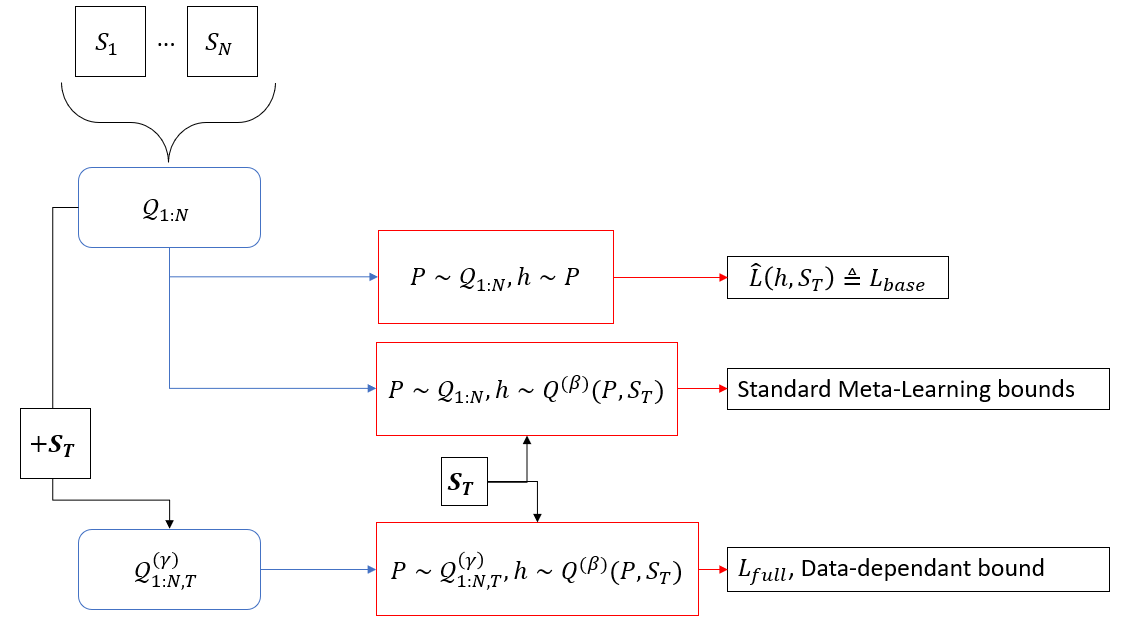
\includegraphics[width=0.9\textwidth]{data_dependant_adaptation.PNG}
	\caption{Flowchart of hyper-posterior construction settings detailing how the test data $S_T$ can be used. A hyper-prior $\mathcal{Q}_{1:N}$ is learned from the training data. This hyper-prior can be sampled and then a hypothesis can be sampled from the resulting prior, thereby ignoring the test data. Standard meta-learning bounds use the test data to adapt the sampled prior before sampling a specific hypothesis. Our approach using data-dependent bounds also applies $S_T$ to the hyper-prior, resulting in a data-dependent hyper-posterior $\mathcal{Q}_{1:N, T}$. }
	\label{fig:data_dependant_bound}
\end{figure}

As we have seen, the meta-learning framework provides us with an informative hyper-posterior from which a good prior (i.e. one with low expected error) can be sampled. Given a specific downstream task $\mathcal{D}_T\sim \tau$ and a sample $S_T\sim \mathcal{D}^m$, we would like to provide a bound on the performance of any hyper-posterior that uses $S_T$ and the given hyper-prior $\mathcal{Q}_{1:N}$ that we previously meta-learned. In order to do so, we make use of PAC-Bayes bounds for data-dependent priors as the $i.i.d$ assumption common to PAC-Bayes bounds may not apply. As such, we re-state a known inequality from \citet{Rivasplata2020} and adapt it to the meta-learning setting:

\begin{theorem} (PAC-Bayes for stochastic kernels - adapted from Theorem 2 in \citet{Rivasplata2020}) \label{thm:rivasplata-pb}
	Let $P\in \mathcal{K}(\mathcal{Z}^m, \mathcal{H})$ be a stochastic kernel, let $A: \mathcal{Z}^m\times \mathcal{H}\rightarrow \mathbb{R}^k$ be a measurable function for some positive integer $k$ and $F:\mathbb{R}^k\rightarrow \mathbb{R}$ be a convex function.
	Define $f\triangleq F\circ A$, and let 
	$$\xi(P_S, \mathcal{D}, f)=\int_{\mathcal{Z}^m}\int_{\mathcal{H}}e^{f(S, h)}P_S(dh)\mathcal{D}(dS)$$
	Such that $P_S$ is the distribution over $\mathcal{H}$ corresponding to the sampled $S$.
	
	Assuming $\xi(P_S, \mathcal{D}, f)$ is finite, for any $\delta \in (0,1)$, the following inequality holds uniformly for all posteriors $Q\in \mathcal{K}(\mathcal{Z}^m, \mathcal{H})$ with probability at least $1-\delta$ over the choice of $S\sim \mathcal{D}$:
	
	\begin{equation} \label{eq:ribasplata-pb}
	\Expect{h\sim Q_S}{f(S, h)} \leq D_{KL}(Q_S||P_S)+\log\left (\frac{\xi(P_S, \mathcal{D}, f)}{\delta}\right )
	\end{equation}
\end{theorem}

The term $\xi(P_S, \mathcal{D}, f)$ is known as the \emph{moment-generating function}, and when it exists, it is an alternative specification of the probability distribution for $f$.
This moment-generating function intuitively quantifies the concentration of the function $f$ in the stochastic kernel $P\in{\cal K}({\cal Z}^m,{\cal H})$, and will be low if $f$ is well-concentrated.
The term $\log\xi(P_S, \mathcal{D}, f)$ is known as the \emph{log-moment}. 
One simple setting where this term can be upper bounded is when the prior $P_S$ is data-free and $f$ is bounded., By switching the order of expectations (Fubini's theorem) and using Hoeffding's lemma, an upper bound for $f(S,h)=\lambda(\mathcal{L}(h,\mathcal{D})-\hat{\mathcal{L}}(h, S))$ for any $\lambda\in \mathbb{R}$ would be:

$$\Expect{h\sim Q_S}{\lambda(\mathcal{L}(h,\mathcal{D})-\hat{\mathcal{L}}(h, S))} \leq D_{KL}(Q_S||P_S)+\log\left (\frac{1}{\delta}\right ) + \frac{\lambda^2(b-a)^2}{8}$$

Notably, this bound is similar to that of \citet{Catoni2004}. Other choices of $f$ result in other traditional PAC-Bayes bounds such as that of \citet{Mcallester} via similar methods (see \citet{Rivasplata2020} for further detail). 
One particularly appealing application of this general bound is for data-dependent priors with bounded log-moment terms, for example by conforming to certain algorithmic stability properties 
As an example for this notion, \citet{Rivasplata2020} show that for any prior satisfying the differential privacy property ($DP(\epsilon)$), the log-moment can be upper bounded by the log-moment of a data-free prior plus a term that depends on the privacy parameter $\epsilon$. \RM{Give ref and examples} \LF{Fixed.}

These data-dependent bounds can be applied to the meta-learning setting, giving us the following general proposition:

\begin{proposition} \label{thm:main-result}
	Let $\mathcal{Q}_{1:N}\in \mathcal{M}(\mathcal{M}(\mathcal{H}))$ be a meta-learned hyper-posterior (e.g. the result of meta-training on $\{S_1,...,S_N\}$), and let $\mathcal{D}_T\sim \tau$ be a \emph{given} test task. Let $Q: \mathcal{Z}^m\times\mathcal{M}(\mathcal{H})\rightarrow \mathcal{M}(\mathcal{H})$ be a given base learner. Let $l: \mathcal{H}\times \mathcal{Z}\rightarrow [0, 1]$ be a bounded loss function.
	For any $\delta_T \in (0,1)$, and for all $\lambda>0$, the following inequality holds uniformly for all hyper-posteriors $\mathcal{Q}\in \mathcal{M}(\mathcal{M}(\mathcal{H}))$ with probability at least $1-\delta_T$ over the draw of $S_T\sim \mathcal{D}_T$:
	
	\begin{align} \label{eq:main-result-generic}
	\mathcal{L}(\mathcal{Q}, \mathcal{D}_T)) \leq \hat{\mathcal{L}}(\mathcal{Q}, S_T) + \frac{1}{\lambda}D_{KL}(\mathcal{Q}||\mathcal{Q}_{1:N})
	+\frac{1}{\lambda}\log\frac{\tilde{\xi}(\lambda,\mathcal{Q}_{1:N},\mathcal{D}_T)}{\delta_T}
	\end{align}
	
	
	where 
	$$\tilde{\xi}(\lambda,\mathcal{Q}_{1:N},\mathcal{D}_T)\triangleq \Expect{S\sim \mathcal{D}_T, P\sim \mathcal{Q}_{1:N}, h\sim Q(P,S)}{e^{\lambda\left (\mathcal{L}(h, \mathcal{D}_T))-\hat{\mathcal{L}}(h, S)\right )}}$$
\end{proposition}

The full proof of Proposition \ref{thm:main-result} is in Appendix \ref{append:proof-main-result}, but it follows quite straightforwardly from Theorem \ref{thm:rivasplata-pb} using a two-level prior hypothesis $(\mathcal{Q}_{1:N}, Q)$, meaning the distribution where we first sample $P\sim \mathcal{Q}_{1:N}$ and then sample $h\sim Q(P, S_T)$ to arrive at a hypothesis. This two-level prior is compared to a two-level posterior $(\mathcal{Q}, Q)$. The proof itself applies even if the loss function $l$ is not bounded, but this assumption is very useful for providing bounds on the log-moment term.

Since the bound allows for a data-dependent prior, it is possible to choose the same base learner $Q(P, S_T)$ for both prior and posterior, resulting in a bound with only an environment-level complexity term. 
Notably, this differs significantly from a more traditional bound that would use a data-free two-level prior $(\mathcal{Q}_{1:N}, P)$. This would result in a bound that contains two complexity terms:

\begin{align*}
\begin{split}
\mathcal{L}(\mathcal{Q}, \mathcal{D}_T)) &\leq \hat{\mathcal{L}}(\mathcal{Q}, S_T) \\
&+ \frac{1}{\lambda}D_{KL}(\mathcal{Q}||\mathcal{Q}_{1:N}) + \frac{1}{\lambda}\Expect{P\sim \mathcal{Q}}{D_{KL}(Q(P,S_T)||P)}\\
&+\frac{1}{\lambda}\log\frac{1}{\delta_T}+\frac{1}{\lambda}\frac{\lambda^2}{8m}
\end{split}
\end{align*}

This more traditional bound contains a task-level complexity term, but since the base learner $P$ is independent from $S_T$ the moment term can be easily bounded. In essence, we can see this as a trade-off between the part of the bound that can be optimized by choosing $\mathcal{Q}$ and the term in the bound that results from the log-moment.

One immediate result of Equation \ref{eq:main-result-generic} is a useful bound on the expected error of the hyper-prior for the downstream task, achieved by picking $\mathcal{Q}=\mathcal{Q}_{1:N}$:

\begin{corollary} \label{thm:corollary-base}
	Let $\mathcal{Q}_{1:N}\in \mathcal{M}(\mathcal{M}(\mathcal{H}))$ be a meta-learned hyper-posterior (e.g. the result of meta-training on $\{S_1,...,S_N\}$), and let $\mathcal{D}_T\sim \tau$ be a \emph{given} test task. Let $Q: \mathcal{Z}^m\times\mathcal{M}(\mathcal{H})\rightarrow \mathcal{M}(\mathcal{H})$ be a given base learner. Let $l: \mathcal{H}\times \mathcal{Z}\rightarrow [0, 1]$ be a bounded loss function.
	For any $\delta_T \in (0,1)$, and for all $\lambda>0$, with probability at least $1-\delta_T$ over the draw of $S_T\sim \mathcal{D}_T$:
	
	$$\mathcal{L}(\mathcal{Q}_{1:N}, \mathcal{D}_T)) \leq \hat{\mathcal{L}}(\mathcal{Q}_{1:N}, S_T)
	+\frac{1}{\lambda}\log\frac{\tilde{\xi}(\lambda,\mathcal{Q}_{1:N},\mathcal{D}_T)}{\delta_T}$$
	
	where 
	$$\tilde{\xi}(\lambda,\mathcal{Q}_{1:N},\mathcal{D}_T)\triangleq \Expect{S\sim \mathcal{D}_T, P\sim \mathcal{Q}_{1:N}, h\sim Q(P,S)}{e^{\lambda\left (\mathcal{L}(h, \mathcal{D}_T))-\hat{\mathcal{L}}(h, S)\right )}}$$
\end{corollary}

It is important to note that the log-moment term $\log\tilde{\xi}(\lambda,\mathcal{Q}_{1:N},\mathcal{D}_T)$ is a key term in both cases. This term will be low if the empirical losses are well concentrated around the expected loss for our data-dependent prior. One possible method of achieving this is by choosing a base learner $Q$ with algorithmic stability properties such as the empirical Gibbs posterior, as we will see in the next subsection.

Unlike the results in Section \ref{sec:meta}, the right-hand side for this bound contains the empirical loss on data from the test task, making straightforward comparison between these bounds effectively impossible. The bound in Corollary \ref{thm:corollary-base} can be thought of as a confidence bound for the expected loss whereas the bound in Theorem \ref{thm:meta-highprob} provides a PAC-Bayes bound based on the data-free hyper-prior and the average training loss.

\subsection{Meta-adaptation with Gibbs posteriors} \label{sec:adapt-gibbs}
%meta-train, meta-test with Gibbs

One class of hyper-posteriors that is especially appealing for analysis given Proposition \ref{thm:main-result} is the class of Gibbs posteriors.

\begin{defn} \label{defn:Gibbs}
	The Gibbs distribution with parameter $\beta>0$ is defined as $$Q(P,S)(h)=\frac{P(h)e^{-\beta \hat{\mathcal{L}}(h,S)}}{Z_\beta(S,P)}$$ 
	where 
	$$Z_\beta(S,P)=\Expect{h\sim P}{e^{-\beta\hat{\mathcal{L}}(h,S)}}$$
\end{defn}

It is well-known that given a specific value for $\lambda$, using Donsker and Varadhan’s variational formula \citep{Donsker1975} provides the hyper-posterior that minimizes the right-hand side of Equation \ref{eq:main-result-generic}:

$$\min_{\mathcal{Q}} \left\{ \hat{\mathcal{L}}(\mathcal{Q}, S_T) + \frac{1}{\lambda}D_{KL}(\mathcal{Q}||\mathcal{Q}_{1:N}) \right\} = \frac{\mathcal{Q}_{1:N}e^{-\lambda\hat{L}(Q,S_T)}}{\Expect{P\sim \mathcal{Q}_{1:N}}{e^{-\lambda\hat{L}(Q,S_T)}}}\triangleq \mathcal{Q}^{\lambda}_{1:N,T}$$

The meaning of this result is that given that we know the relative importance of the empirical loss and the KL-divergence, the optimal hyper-posterior is the Gibbs hyper-posterior $\mathcal{Q}^{\lambda}_{1:N,T}$.

This property encourages further exploration of the Gibbs hyper-posterior for meta-adaptation. We define $$\mathcal{Q}^{\gamma}_{1:N,T}\triangleq \frac{\mathcal{Q}_{1:N}e^{-\gamma\hat{\mathcal{L}}(Q(P,S_T),S_T)}}{Z_\gamma(S_T, \mathcal{Q}_{1:N})}$$ as the Gibbs posterior for the meta-learned problem with meta-normalization term $$Z_\gamma(S_T, \mathcal{Q}_{1:N})=\Expect{P\sim \mathcal{Q}_{1:N}}{e^{-\gamma\hat{\mathcal{L}}(Q(P,S_T),S_T)}}.$$

We have 
$$KL(\mathcal{Q}^{\gamma}_{1:N,T}||\mathcal{Q}_{1:N})=
-\gamma\hat{\mathcal{L}}(\mathcal{Q}_{1:N,T}, S_T)-\log\Expect{P\sim \mathcal{Q}_{1:N}}{e^{-\gamma\hat{\mathcal{L}}(Q(P,S_T),S_T)}}$$ 

So by plugging these values in Equation \ref{eq:main-result-generic} gives us
\begin{align*} 
\begin{split}
\mathcal{L}(\mathcal{Q}^{\gamma}_{1:N,T}, \mathcal{D}_T)) & \leq \hat{\mathcal{L}}(\mathcal{Q}^{\gamma}_{1:N,T}, S_T) -\frac{\gamma}{\lambda}\hat{\mathcal{L}}(\mathcal{Q}^{\gamma}_{1:N,T}, S_T) \\ &- \frac{1}{\lambda}\log\Expect{P\sim \mathcal{Q}_{1:N}}{e^{-\gamma\hat{\mathcal{L}}(Q(P,S_T),S_T)}}\\ &+\frac{1}{\lambda}\log\frac{\tilde{\xi}(\lambda,\mathcal{Q}_{1:N},\mathcal{D}_T)}{\delta_T}
\end{split}
\end{align*}

In order to clarify this expression, we will use more intuitive definitions for our empirical losses:
\begin{defn}
	We define the adapted meta-loss (AML) $$\hat{\mathcal{L}}_{aml}\triangleq \hat{\mathcal{L}}^{(\gamma,\beta)}(\mathcal{Q}^{\gamma}_{1:N,T}, S_T)=\mathbb{E}_{P\sim \mathcal{Q}^{\gamma}_{1:N,T}}\mathbb{E}_{h\sim Q^{\beta}(P,S_T)}\left [\hat{\mathcal{L}}(h, S_T)\right ]$$ as the fully adapted loss, meaning $S_T$ is used to adapt both the hyper-prior ($\mathcal{Q}_{1:N}$) and the sampled prior. $\hat{\mathcal{L}}_{aml}$ is a function of both $\gamma$ and $\beta$. 
	
	We define the standard meta-loss $$\hat{\mathcal{L}}_{ml}\triangleq \hat{\mathcal{L}}'(\mathcal{Q}_{1:N}, S_T)=\mathbb{E}_{P\sim \mathcal{Q}_{1:N}}\mathbb{E}_{h\sim Q^{\beta}(P,S_T)}\left [\hat{\mathcal{L}}(h, S_T)\right ]$$ as the empirical loss of the base learner using the hyper-prior. $\hat{\mathcal{L}}_{ml}$ depends on $\beta$, but is not a function of $\gamma$.
\end{defn}

For brevity, we will omit the $\gamma$ from $\mathcal{Q}^{\gamma}_{1:N,T}$ and $\beta$ from $Q^{\beta}$. Using these definitions, we have:

$$\mathcal{L}(\mathcal{Q}_{1:N,T}, \mathcal{D}_T)) \leq \hat{\mathcal{L}}_{aml} -\frac{\gamma}{\lambda}\hat{\mathcal{L}}_{aml} - \frac{1}{\lambda}\log \mathbb{E}_{P\sim \mathcal{Q}_{1:N}}\left [e^{-\gamma\hat{\mathcal{L}}(Q(P,S_T),S_T)}\right ]+\frac{1}{\lambda}\log\frac{\tilde{\xi}(\lambda,\mathcal{Q}_{1:N},\mathcal{D}_T)}{\delta_T}$$

By simplifying the third term using Jensen's inequality , we get:

\begin{equation} \label{eq:pb-adapt-multi}
\mathcal{L}(\mathcal{Q}_{1:N,T}, \mathcal{D}_T)) \leq 
(1-\frac{\gamma}{\lambda})\hat{\mathcal{L}}_{aml} + \frac{\gamma}{\lambda}\hat{\mathcal{L}}_{ml} 
+\frac{1}{\lambda}\log\frac{\tilde{\xi}(\lambda,\mathcal{Q}_{1:N},\mathcal{D}_T)}{\delta_T}
\end{equation}

This equation gives us a generalization bound that considers the empirical loss of the hyper-prior as well as the empirical loss for the posterior, thereby giving us the following theorem:

\begin{corollary} \label{thm:main-result-gibbs}
	Let $\mathcal{Q}_{1:N}$ be a hyper-posterior (e.g. the result of meta-training on $\{S_1,...,S_N\}$), and let $\mathcal{D}_T\sim \tau$ be a given test task. Let $$\mathcal{Q}_{1:N,T}= \frac{\mathcal{Q}_{1:N}e^{-\gamma\hat{\mathcal{L}}(Q(P,S_T),S_T)}}{Z_\gamma(S_T, \mathcal{Q}_{1:N})}$$ be the empirical Gibbs distribution for given dataset $S_T\sim \mathcal{D}_T$.
	
	For all $\lambda>0, \gamma>0$, 
	with probability at least $1-\delta_T$ over the draw of $S_T\sim \mathcal{D}_T$:
	
	$$\mathcal{L}(\mathcal{Q}_{1:N,T}, \mathcal{D}_T)) \leq 
	(1-\frac{\gamma}{\lambda})\hat{\mathcal{L}}_{aml} + \frac{\gamma}{\lambda}\hat{\mathcal{L}}_{ml} 
	+\frac{1}{\lambda}\log\frac{\tilde{\xi}(\lambda,\mathcal{Q}_{1:N},\mathcal{D}_T)}{\delta_T}$$
\end{corollary}

In order to better understand the impact of the log-moment term, we remark that \citet{Rivasplata2020} have shown that for $\lambda=\sqrt{m}$ and given that the base learner is the empirical Gibbs posterior $Q^\beta$ and the loss is bounded:

$$\log\tilde{\xi}(\sqrt{m},\mathcal{Q}_{1:N},\mathcal{D}_T) \leq 2+\log(1+\sqrt{e})+\frac{2\beta}{\sqrt{m}} $$

As a consequence of this, choosing $\beta=\sqrt{m}$ would result in a bound on the generalization gap of rate $O(\frac{1}{\sqrt{m}})$.

Corollary \ref{thm:main-result-gibbs} provides an upper bound on the expected error for a given test task that depends on the empirical errors of the hyper-prior $\hat{\mathcal{L}}_{ml}$ and the hyper-posterior $\hat{\mathcal{L}}_{aml}$. 
Since the bound applies uniformly for all $\gamma>0,\beta>0,\lambda>0$, this bound can be further optimized by choosing optimal values for $\gamma, \beta, \lambda$. This can be done by deriving the right-hand-side of Equation \ref{eq:pb-adapt-multi} and comparing to zero. 
We show the derivation itself in Appendix \ref{append:optimiziation}, and provide the end result here:

\begin{align} \label{eq:meta-pb-gamma-paper}
\begin{split}
\gamma = \lambda+\frac{\hat{\mathcal{L}}_{ml}-\hat{\mathcal{L}}_{aml}}{\frac{d}{d\gamma}\hat{\mathcal{L}}_{aml}}
\end{split}\hfill
\end{align}

\begin{align} \label{eq:meta-pb-lambda-paper}
\begin{split}
\lambda = \frac{\gamma(\hat{\mathcal{L}}_{ml}-\hat{\mathcal{L}}_{aml})+\log\frac{\tilde{\xi}(\lambda,\mathcal{Q}_{1:N},\mathcal{D}_T)}{\delta_T}}{\frac{d}{d\lambda}\log\tilde{\xi}(\lambda,\mathcal{Q}_{1:N},\mathcal{D}_T)}
\end{split}
\end{align}

Equation \ref{eq:meta-pb-gamma-paper} encourages an equilibrium for $\gamma$, as a negative value of $\hat{\mathcal{L}}_{ml}-\hat{\mathcal{L}}_{aml}$ (meaning the meta-adaptation is harmful) encourages increasing $\gamma$, and a positive value encourages lowering $\gamma$.
This result aligns well with Equation \ref{eq:pb-adapt-multi}, since if the adapted loss is low we are encouraged to decrease $\gamma$ to tighten the bound, but that would lead to the hyper-posterior to be more similar to the hyper-prior, and similarly if the base loss $\hat{\mathcal{L}}_{ml}$ is low we are encouraged to increase $\gamma$ in order to tighten the bound.

Equation \ref{eq:meta-pb-lambda-paper} contains the log-moment term, thereby preventing the choice of a large $\lambda$ that would cause the moment to diverge. Aside from that term, 
the first term of the numerator serve encourages a lower value for $\lambda$ if there is a positive prediction gain from meta-adaptation $\hat{\mathcal{L}}_{aml}<\hat{\mathcal{L}}_{ml}$.

\subsection{Tighter bounds for the low error setting}
% seeger

Corollary \ref{thm:main-result} is the result of applying the generic data-dependent bound (Theorem \ref{thm:rivasplata-pb}) with the measurement function $f=\lambda(\mathcal{L}(\mathcal{Q},\mathcal{D}_T))-\hat{\mathcal{L}}(\mathcal{Q}, S_T))$. For cases where $\hat{\mathcal{L}}(\mathcal{Q}, S_T)$ is low, it may be better to use a bound based on the binary KL-divergence: $f=\lambda kl(\hat{\mathcal{L}}(\mathcal{Q}, S_T)||\mathcal{L}(\mathcal{Q},\mathcal{D}_T)))$
where $$kl(q||p)=q \log\frac{q}{p}+(1-q)\log\frac{1-q}{1-p}, q,p\in[0, 1]$$

Doing so gives the upper bound:

\begin{align} \label{eq:generic-kl-bound}
kl(\hat{\mathcal{L}}(\mathcal{Q}, S_T)||\mathcal{L}(\mathcal{Q},\mathcal{D}_T))) \leq \frac{1}{\lambda}\left (D_{KL}(\mathcal{Q}||\mathcal{Q}_{1:N})+\log\frac{\bar{\xi}(\mathcal{Q}_{1:N}, \mathcal{D}_T,\lambda, kl)}{\delta_T} \right )
\end{align}

One useful inequality for converting this bound to one with a more similar structure to previously discussed bounds is an inequality used by \citet{Tolstikhin2013}:

\begin{lemma} \citep{Tolstikhin2013} \label{thm:kl-inverse}
	For 1-dimensional random variables $p,q \in [0, 1]$,
	$$kl^-1(q||p)\leq q + \sqrt{2qp}+2p$$
\end{lemma}

Using Lemma \ref{thm:kl-inverse} on the upper bound gives the following upper bound:

\begin{align} \label{eq:tolstikhin-kl-bound}
\begin{split}
\mathcal{L}(\mathcal{Q},\mathcal{D}_T)) &\leq \hat{\mathcal{L}}(\mathcal{Q}, S_T) + 2\frac{D_{KL}(\mathcal{Q}||\mathcal{Q}_{1:N})+\log\frac{\xi(\mathcal{Q}_{1:N}, \mathcal{D}_T,\lambda, kl)}{\delta_T}}{\lambda}\\
&+\sqrt{2\hat{\mathcal{L}}(\mathcal{Q}, S_T)\frac{D_{KL}(\mathcal{Q}||\mathcal{Q}_{1:N})+\log\frac{\xi(\mathcal{Q}_{1:N}, \mathcal{D}_T,\lambda, kl)}{\delta_T}}{\lambda}}
\end{split}
\end{align}

Another interesting variation of Equation \ref{eq:generic-kl-bound} is if the base learner $Q$ is the Gibbs posterior, as the moment term can be meaningfully bounded. To do so, we make use of the differential privacy traits of the Gibbs posterior.

\begin{defn} (Differential privacy)
	Let $S,S'\in \mathcal{Z}^m$ be datasets that differ by a single element.
	A randomized algorithm $\mathcal{A}$ is called  $\epsilon$-differentially private, marked $DP(\epsilon)$ if for any $I\subset image(\mathcal{A})$:
	
	$$Pr(\mathcal{A}(S)\in I)\leq e^\epsilon Pr(\mathcal{A}(S')\in I)$$
\end{defn}

An equivalent definition for stochastic kernels that is easier to understand for our setting is:

\begin{defn} (Differential privacy)
	Let $S,S'\in \mathcal{Z}^m$ be datasets that differ by a single element.
	Let $Q\in \mathcal{K}(\mathcal{Z}^m, \mathcal{M}(\mathcal{H}))$ be a stochastic kernel.
	$Q$ is $DP(\epsilon)$ if 
	
	$$\frac{Q(S, A)}{Q(S', A)} \leq e^\epsilon$$
	
	For all $A\in  \mathcal{M}(\mathcal{H})$
\end{defn}

It has been proven \citep{McSherry2007, Rivasplata2020} that the Gibbs posterior $Q(P, S)(h)\propto P(h)e^{-\beta\hat{\mathcal{L}}(h, S)}$ is $DP\left (\frac{2\beta}{m}\right )$.
This result can be extended to the meta-learning setting as follows:

\begin{proposition} \label{thm:pair-is-dp}
	Let $\mathcal{P}\in \mathcal{M}(\mathcal{M}(\mathcal{H}))$ be a hyper-prior.
	Let $l:\mathcal{H}\times \mathcal{Z}\rightarrow [0,1]$ be a bounded loss function.
	
	If the base learner $Q\in \mathcal{M}(\mathcal{H})$ is the Gibbs posterior $Q(P, S)(h)\propto P(h)e^{-\beta\hat{\mathcal{L}}(h, S)}$, 
	then the pair hypothesis $(\mathcal{P}, Q)$ satisfies $DP\left (\frac{2\beta}{m}\right )$.
\end{proposition}

The proof of Proposition \ref{thm:pair-is-dp} is in Appendix \ref{append:proof-dp}. This  allows us to extend an existing result for PAC-Bayes with private data-dependent priors:

\begin{theorem} (Theorem 4.2 in \citet{Dziugaite2018})
	Let $l:\mathcal{H}\times \mathcal{Z}\rightarrow [0,1]$ be a bounded loss function.
	Let $\mathbb{P}:\mathcal{Z}\rightarrow \mathcal{M}(\mathcal{H})$ be an $\epsilon$-differentially private algorithm for choosing a prior.
	
	The following inequality holds uniformly for all posteriors $Q\in \mathcal{M}(\mathcal{H})$ with probability at least $1-\delta$ over the draw of $S\sim \mathcal{D}$:
	
	$$kl(\hat{\mathcal{L}}(Q,S)||\mathcal{L}(\mathcal{D},S))\leq \frac{1}{m}\left (D_{KL}(Q||\mathbb{P}(S))+\log\frac{4\sqrt{m}}{\delta} \right ) +\frac{\epsilon^2}{2}+\epsilon\sqrt{\frac{\log (4/\delta)}{2m}} $$

\end{theorem}

\begin{corollary} \label{thm:kl-main-result}
	Let $l:\mathcal{H}\times \mathcal{Z}\rightarrow [0,1]$ be a bounded loss function.
	Let $\mathcal{Q}_{1:N}$ be a hyper-posterior (e.g. the result of meta-training on $\{S_1,...,S_N\}$), and let $\mathcal{D}_T\sim \tau$ be a given test task. 
	
	If the base learner $Q\in \mathcal{M}(\mathcal{H})$ is the Gibbs posterior $Q(P, S)(h)\propto P(h)e^{-\beta\hat{\mathcal{L}}(h, S)}$, 
	The following inequality holds uniformly for all hyper-posteriors $\mathcal{Q}\in \mathcal{M}(\mathcal{M}(\mathcal{H}))$ with probability at least $1-\delta$ over the draw of $S_T\sim \mathcal{D}_T$:
	
	$$kl(\hat{\mathcal{L}}(\mathcal{Q},S)||\mathcal{L}(\mathcal{Q},S))\leq \frac{1}{m}\left (D_{KL}(\mathcal{Q}||\mathcal{Q}_{1:N})+\log\frac{4\sqrt{m}}{\delta_T} \right ) +2\frac{\beta^2}{m^2}+\frac{\beta}{m}\sqrt{\frac{2\log (4/\delta_T)}{m}} $$
	
\end{corollary}

Choosing $\beta=\sqrt{m}$ results in the right-hand side of this Corollary to have rate $O\left (\frac{1}{m}\right )$, and as we have seen before in Equation \ref{eq:tolstikhin-kl-bound}, for the realizable setting this results in rate $O\left (\frac{1}{m}\right )$ for the expected loss as well.

%\subsection{Oracle bounds for meta-learning and adaptation}
% oracle

%Another possible use of the Gibbs posterior is to provide oracle bounds 



%\section{Optimal Meta-adaptation with stable base learners}

%We note that Equation \ref{eq:generic-adapt-bound} applies for any hyper-posterior, since it is derived before using the specific choice of hyper-posterior. Therefore, for any $\mathcal{Q}$ (with probability at least $1-\delta_T$):
%
%$$\mathcal{L}(\mathcal{Q}, \mathcal{D}_T)) \leq \hat{\mathcal{L}}(\mathcal{Q}, S_T) + \frac{1}{\lambda}D_{KL}(\mathcal{Q}||\mathcal{Q}_{1:N})+\frac{1}{\lambda}ln\frac{\xi(\lambda,\mathcal{Q}_{1:N})}{\delta_T}$$
%
%Since the log-moment term $ln\xi(\mathcal{Q}_{1:N}, \lambda)$ does depend on the hyper-posterior, for a given value of $\lambda>0$, we can optimize the right-hand side:
%
%$$\mathcal{Q}^*_\lambda=\min_{\mathcal{Q}} \left\{ \hat{\mathcal{L}}(\mathcal{Q}, S_T) + \frac{1}{\lambda}D_{KL}(\mathcal{Q}||\mathcal{Q}_{1:N}) \right\}$$
%
%% TODO: ref
%Using Donsker and Varadhan’s variational formula \cite{???}, finding the optimal value $\mathcal{Q}^*_\lambda$ is simple, and in fact it is the Gibbs hyper-posterior:
%
%$$\mathcal{Q}^*_\lambda(P)=\frac{\mathcal{Q}_{1:N}e^{-\lambda\hat{L}(Q,S_T)}}{\Expect{P\sim \mathcal{Q}_{1:N}}{e^{-\lambda\hat{L}(Q,S_T)}}}$$
%
%\LF{This is pretty well-known in PB literature, but maybe prove this in an appendix?}

%This variation on the bound gives us a the following version of the bound from Theorem \ref{thm:main-result}:
%
%$$\mathcal{L}(\mathcal{Q}^*_\lambda, \mathcal{D}_T)) \leq \mathcal{L}_{noadapt} + \frac{1}{\lambda}ln\frac{\xi(\lambda,\mathcal{Q}_{1:N})}{\delta_T}$$
%
%% TODO: proof
%This bound on the expected loss of $\mathcal{Q}^*_\lambda$ essentially depends entirely on the hyper-prior $\mathcal{Q}_{1:N}$. We note that if $\lambda=O(\sqrt{m})$, it is possible (see Appendix \ref{???}) to extend Lemma 3 in Appendix B of \citet{Rivasplata2020} to show that if the loss function $l$ is upper bounded by a constant $b$, then:
%
%$$ln\xi(\mathcal{Q}_{1:N}, \sqrt{m}) \leq 2b^2(1+\frac{2\gamma}{\sqrt{m}})+log(1+e^{b^2/2})$$
%
%Giving us
%
%\begin{theorem} \label{thm:optimal-adaptation-bound}
%	Let $\mathcal{Q}_{1:N}$ be a hyper-posterior (e.g. the result of meta-training on $\{S_1,...,S_N\}$), and let $\mathcal{D}_T\sim \tau$ be a given test task. Choose $\lambda>0$. Let $$\mathcal{Q}^*_\lambda= \frac{\mathcal{Q}_{1:N}e^{-\lambda\hat{\mathcal{L}}(Q(P,S_T),S_T)}}{Z_\gamma(S_T, \mathcal{Q}_{1:N})}$$ be the empirical Gibbs distribution for given dataset $S_T\sim \mathcal{D}_T$.
%	
%	With probability at least $1-\delta_T$ over the draw of $S_T\sim \mathcal{D}_T$:
%	
%	$$\mathcal{L}(\mathcal{Q}^*_\lambda, \mathcal{D}_T)) \leq 
%	 \hat{\mathcal{L}}_{ml} 
%	+\frac{1}{\sqrt{m}}\left (6b^2+ln\frac{1+e^{b^2/2}}{\delta_T}\right )$$
%\end{theorem}
%
%This specific choice of parameters gives us an upper bound on the expected loss of the meta-adapted hyper-posterior in terms of the empirical loss of our given hyper-prior $\mathcal{Q}_{1:N}$ and the size of the adaptation set $m$. 
%Sadly, this result does not yield any novel insights on constructing $\mathcal{Q}_{1:N}$, as it only tells us that a learned hyper-prior that would perform well on samples from new tasks is expected to generalize well on those tasks. 

%\LF{Interesting direction: this bound is vacuous for few-shot adaptation ($\sqrt{m}<6b^2$), it seems that the few shot adaptation setting requires either very low $\lambda$ (since we can use existing bounds from the training data) or very high $\lambda$ (weak reliance on the prior, but may cause the moment to diverge)}

\section{Theoretical and empirical comparison of bounds}

%TODO: cleanup

In order to better understand the differences between the classical bound and this novel meta-adaptation bound, we consider a simple comparison setting. We take four regression tasks with data from 2D-Gaussian distributions each with different means. 
For each task, we sample 1000 examples in total.
Figure \ref{fig:ex-baseline} shows the training tasks and the hyper-posterior $\mathcal{Q}_{1:4}$ learned from them (modeled as a 2D-Gaussian over priors).

\begin{figure}
	\centering
	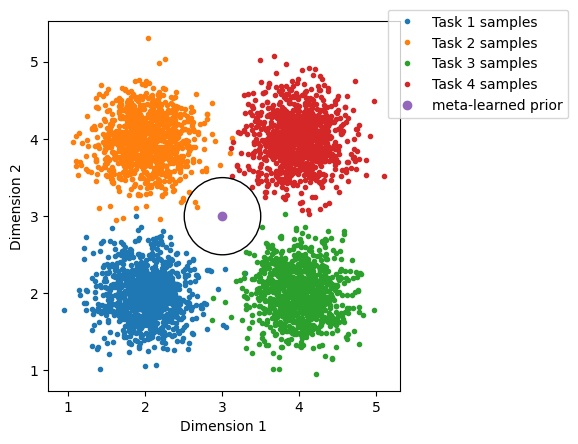
\includegraphics[width=0.9\textwidth]{toy_example_train.JPG}
	\caption{Four training tasks and the learned hyper-posterior $\mathcal{Q}_{1:4}$}
	\label{fig:ex-baseline}
\end{figure}

We consider the test performance of this hyper-posterior on a new test task $\mathcal{D}_T$, 
which in this case is out-of-distribution but this dies not significantly change the analysis. Figure \ref{fig:ex-erm} shows the result of minimizing the empirical loss on a sampled test set $S_5$ (i.e. running ERM starting from a prior sampled from the hyper-prior $P\sim \mathcal{Q}_{1:4}$). We see that for this simple setting, the empirical loss for the posterior is low, as there is sufficient data to learn the new task.
While ERM is effective as a base learner here, using an objective inspired by PAC-Bayes bound such as $$\min_{Q}\hat{\mathcal{L}}(Q, S_T) + \frac{1}{\lambda}KL(Q||P)$$ would also lead to similar results. 

\begin{figure}
	\centering
	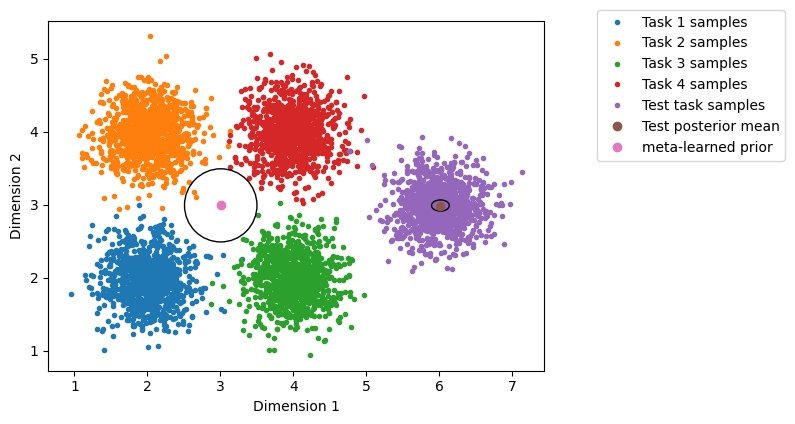
\includegraphics[width=0.9\textwidth]{toy_example_erm.JPG}
	\caption{Transfer of a learned hyper-prior $\mathcal{Q}_{1:4}$ to a new task with ERM}
	\label{fig:ex-erm}
\end{figure}


We now show the result of applying a simple meta-adaptation objective: 
$$\min_{Q}\hat{\mathcal{L}}(Q, S_T) + \frac{1}{\lambda}\Expect{P\sim \mathcal{Q}}{KL(Q||P)}+\frac{1}{\lambda}KL(\mathcal{Q}||\mathcal{Q}_{1:4})$$
Notably, the task prior $P$ is sampled from $\mathcal{Q}$. Figure \ref{fig:ex-aml} shows the adaptation process as well as the final result. We see that this objective yields a hyper-posterior $\mathcal{Q}$ with a closer mean to the test task, and we see that the variance of the prior is high along the axis connecting the hyper-prior and the test posterior. 

\begin{figure}[h!]
	\centering
	\begin{subfigure}[b]{0.49\textwidth}
		\centering
		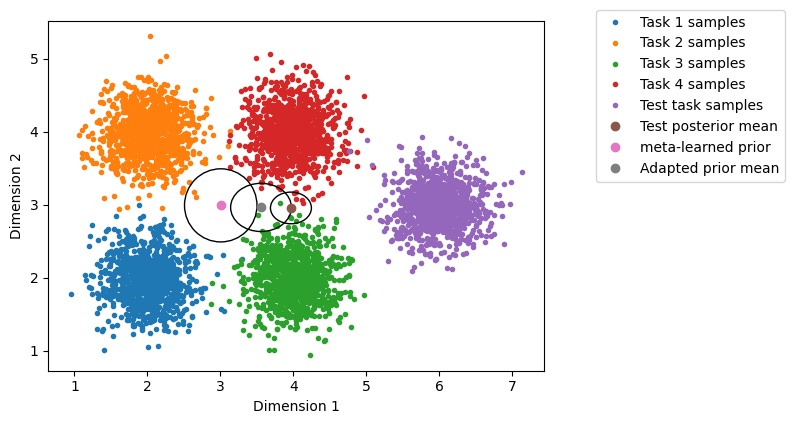
\includegraphics[width=\textwidth]{toy_example_aml_mid.JPG}
		\caption{Meta-adaptation after 10 SGD steps.}
	\end{subfigure}
	\hfill
	\begin{subfigure}[b]{0.49\textwidth}
		\centering
		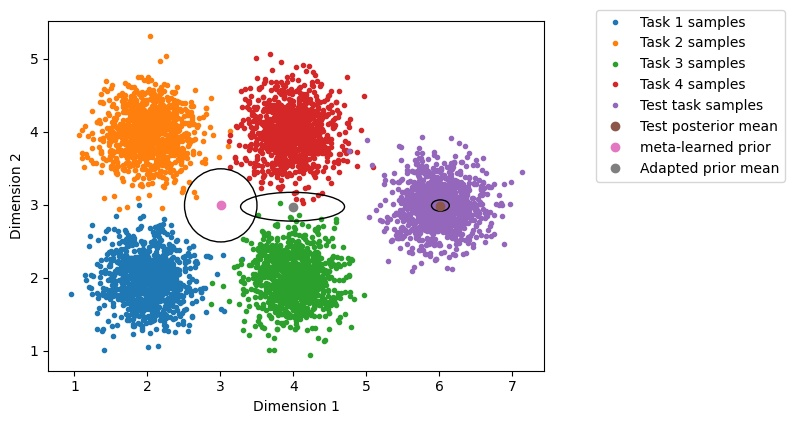
\includegraphics[width=\textwidth]{toy_example_aml_fin.JPG}
		\caption{Meta-adaptation after convergence.}	 	
	\end{subfigure}
	\hfill
	\caption{Adaptation and transfer from a learned hyper-prior to a new task}	 
	\label{fig:ex-aml}
\end{figure}

Since the empirical loss of the final hypothesis is similar regardless of hyper-prior, we can easily compare the bounds. We will mark this empirical loss $\hat{l}$. Since the number of samples per task $m$ is quite large ($m=1000$), terms that are divided by it are small. For the training-based bound of Equation \ref{eq:meta-pb-amit}, we have (with probability at least $1-\delta$ over the choice of $S_1,...,S_4$ and probability at least $1-\delta_T$ over the choice of $S_T$):

\begin{align*}
\begin{split}
	\mathcal{L}(\mathcal{Q}_{1:4},\mathcal{D}_T)\leq \hat{l} &+ \sqrt{\frac{D_{KL}(\mathcal{Q}_{1:4}||\mathcal{P})+\log\frac{2N}{\delta}}{2(N-1)}}
	+O\left (\frac{\sqrt{\log{1/\delta_T}}}{\sqrt{m}}+\frac{\sqrt{\log{m/\delta}}}{\sqrt{m}}\right )
\end{split}
\end{align*}

Where the terms that depend on $\sqrt{m}$ are negligible in comparison to term that depend on the number of tasks $N$.
A quick glance at the meta-adaptation bound of Equation \ref{eq:main-result-generic} shows us that we have for $\lambda=\sqrt{m}$ (with probability at least $1-\delta_T$ over the choice of $S_T$):

\begin{align*}
\begin{split}
\mathcal{L}(\mathcal{Q},\mathcal{D}_T)\leq \hat{l} + O\left (\frac{\sqrt{\log{1/\delta_T}}}{\sqrt{m}}\right ) 
\end{split}
\end{align*}

This comparison lets us clearly see that for a small, finite number of training task, this bound offers significant advantages. We also note that in this example,  $$D_{KL}(\mathcal{Q}_{1:4}||\mathcal{P})>D_{KL}(\mathcal{Q}||\mathcal{Q}_{1:4})$$ 
and so there is an additional advantage in the hyper-KL term being smaller and eliminating the task-level KL terms. This example also shows us that if the empirical loss on the adaptation set $\hat{\mathcal{L}}(\mathcal{Q}, S_T)$ is high, the new meta-adaptation bound is less useful compared to traditional training-set bounds. 

Finally, we note that the choice of $\lambda=\sqrt{m}$ leads to a hyper-posterior that balances low loss with similarity to the hyper-prior, and choosing a significantly higher value may lead to a hyper-prior that coincides with the ERM posterior. Empirically for this setting, choosing $\lambda>>m$ caused this behavior to occur.

\section{Practical implementation and empirical evaluation}

As is usually the case with PAC-Bayes bounds, Theorem \ref{thm:main-result-gibbs} provides us with a practical algorithm for meta-adaptation. In order to perform approximate posterior sampling for a Gibbs posterior, the SGLD (Stochastic Gradient Langevin Dynamics) algorithm \citep{Welling2011} can be used, assuming a sufficient number of iterations.
Combined with Monte-Carlo sampling to estimate expectations over priors, 
this approximation allows for the derivation of a complete practical algorithm for approximating $\mathcal{Q}_{1:N,T}$, which we describe in Algorithm \ref{alg1}.

\begin{algorithm}[H]
	\caption{Meta-adaptation and meta-testing}
	\label{alg1}
	\small
	\begin{algorithmic}
		\Function{Meta-adapt}{$\mathcal{Q}_{1:N}$, $S_T\sim \mathcal{D}_T$,$\beta$}
		\State Initialize $\gamma, \lambda$ to some initial value 
		\State Initialize $\hat{\mathcal{Q}}_{1:N, T}\leftarrow \mathcal{Q}_{1:N}$
		\State Estimate $\hat{\mathcal{L}}_{ml}$
		\While {$\gamma, \lambda$ not converged}
			\State gradients $\leftarrow \emptyset$
			\For {each Monte-Carlo estimation}
				\State Sample $P\sim \hat{\mathcal{Q}}_{1:N, T}$
				\State $h\leftarrow$ \Call{SGLD}{$P$, $S_T$, $\beta$} \Comment Approximate posterior sampling
				\State add $\nabla_{\theta_i} \hat{\mathcal{L}}(h, S_T)$ to gradients
			\EndFor
			\State $\nabla_\theta \hat{\mathcal{L}}(\hat{\cal Q}_{1:N,T}, S_T)\leftarrow$average(gradients)
			\State $\hat{\mathcal{Q}}_{1:N, T}\leftarrow$ \Call{SGLD-step}{$\hat{\mathcal{Q}}_{1:N, T}$, $\gamma$, $\nabla_\theta \hat{\mathcal{L}}(\hat{\cal Q}_{1:N,T}, S_T)$} \Comment Update hyper-posterior
			
			\State Estimate $\hat{\mathcal{L}}_{aml}$
			\State Update $\gamma$ using Equation \ref{eq:meta-pb-gamma}
			\State Update $\lambda$ using Equation \ref{eq:meta-pb-lambda}
			
		\EndWhile
		\State \Return $\hat{\mathcal{Q}}_{1:N, T}$
		\EndFunction
		
		\Function{Meta-test}{$\mathcal{Q}_{1:N,T}$, $S_T\sim \mathcal{D}_T$, $\beta$} 
		\State Sample $P\sim \hat{\mathcal{Q}}_{1:N, T}$
		\State $h\leftarrow$ \Call{SGLD}{$P$, $S_T$, $\beta$} \Comment Sampling $h\sim P$ and using SGD is also valid
		\State Estimate test accuracy $\mathcal{L}_{01}(h, \mathcal{D}_T)$ using held-out test set
		\State \Return accuracy
		\EndFunction
	\end{algorithmic}
\end{algorithm}

Optimizing for $\lambda$ is computationally infeasible in general, as it requires deriving the log-moment term $\log\tilde{\xi}$. Since $\tilde{\xi}(\lambda, \mathcal{Q}_{1:N},\mathcal{D}_T)$ contains an expectation over samples from the underlying test distribution $\mathcal{D}_T$, we cannot derive it directly. As such, we opted to keep $\lambda$ constant, and focused on adapting only the Gibbs temperature parameter $\gamma$.
Estimating $\hat{\mathcal{L}}_{ml},\hat{\mathcal{L}}_{aml}$ is quite simple, but estimating $\frac{d}{d\gamma}\hat{\mathcal{L}}_{aml}$ is a bit more challenging.

Since we tested our approach on neural networks, the hypothesis space is defined as $\{h_w|w\in \mathbb{R}^d\}$ where the weights $w$ serve as the parameters of each hypothesis.
Using the chain rule, 
$$\frac{d}{d\gamma}\hat{\mathcal{L}}_{aml}=\frac{d}{dw}\hat{\mathcal{L}}_{aml}\frac{d}{d\gamma}w$$
Since the update rule of SGLD is 
$$w^{t+1}=w^t-\eta\nabla_w \hat{\mathcal{L}}(h_w,S)+\sqrt{\frac{\eta}{\gamma}}\epsilon \text{ , where } \epsilon\sim N(0,1)$$
We have
\begin{equation}
\frac{d}{d\gamma}w^{t+1}=\frac{d}{d\gamma}w^t-\eta\frac{d}{d\gamma}\nabla_w \hat{\mathcal{L}}(h_w,S)-\frac{1}{2}\sqrt{\frac{\eta}{\gamma^3}}\epsilon
\end{equation}

Since $\frac{d}{d\gamma}w^0=0$, the only remaining issue is deriving the loss gradient by $\gamma$. In our experiments, we assumed $\frac{d}{d\gamma}\nabla_w \hat{\mathcal{L}}(h_w,S)=0$ to simplify the update rule, and if the loss gradient itself is small, this is quite reasonable.

In order to demonstrate the efficacy of our meta-adaptation algorithm, we compare our approach to standard meta-testing for few-shot image classification tasks. 
We use the cross-entropy loss during adaptation, despite the fact that it is not bounded. We note that a clipped variation of this loss does exist and conforms to theoretical guarantees, and in practice the cross-entropy loss tends to be low.

We conduct experiments on a task environment based on the MNIST dataset \citep{LeCun1998}, where each task was created by performing a random permutation on some of the image pixels. The number of pixels to be permuted and the total number of classes (referred to as ``ways'') was chosen in advance. We meta-learn a hyper-prior by running MAML \citep{Finn2017} for 100 meta-training iterations on randomly sampled training tasks, with 10 examples from each class. The resulting network weights were then used as the mean of a d-dimensional Gaussian (with variance $\sigma I_d$, where $\sigma=\sqrt{\frac{\eta}{\gamma}}$ is the noise variance for SGLD) to form our final meta-training hyper-prior $\mathcal{Q}_{1:N}$. We used the same convolutional neural network (CNN) architecture used by \citet{Vinyals2016} for the Omniglot dataset, as it has similar dimensions. We perform our tests on tasks with 100 permuted pixels and compare hyper-priors learned with training tasks that have either 100 or 1000\footnote{Since images in the MNIST dataset have $28\times 28=784$ pixels, this means that there is a high likelihood that most pixels were permuted.} permuted pixels during training. See appendix \ref{append:hyper-params} for a full list of hyper-parameters and implementation details. Code to reproduce our experiments is available at the following \hyperlink{Github repository}{https://github.com/lioritan/phd-work}.

\LF{TODO: move code to a clean github repo, and make wandb optional}

For standard meta-testing, we used SGD with the Adam optimizer \citep{Kingma2015}, and performed 10 adaptation steps given the labeled adaptation dataset $S_T$. For our meta-adaptation method, we utilize a similar setup, but additionally perform 10 steps of meta-adaptation as detailed in Algorithm \ref{alg1} with both pre-selected values for $\gamma$ as well as adapting $\gamma$ using the chain rule decomposition detailed above. Figure \ref{fig:results-gamma} shows the test accuracy averaged over 10 meta-testing seeds for the best hyper-parameters with varying adaptation set sizes. The best accuracies are also reported in Table \ref{table:gamma}.

%TODO: have each plot contain both bad prior and good prior

\begin{figure}[h!]
	\centering
	\begin{subfigure}[b]{0.49\textwidth}
		\centering
		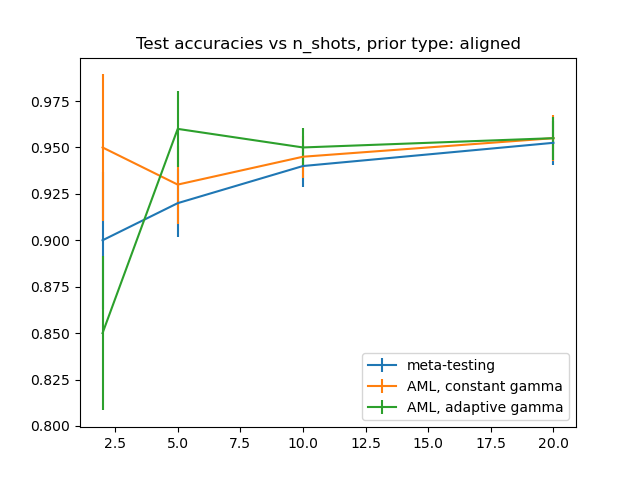
\includegraphics[width=\textwidth]{test_accuracies_model_aligned}
		\caption{Test adaptation for a correct hyper-prior}
	\end{subfigure}
	\hfill
	\begin{subfigure}[b]{0.49\textwidth}
		\centering
		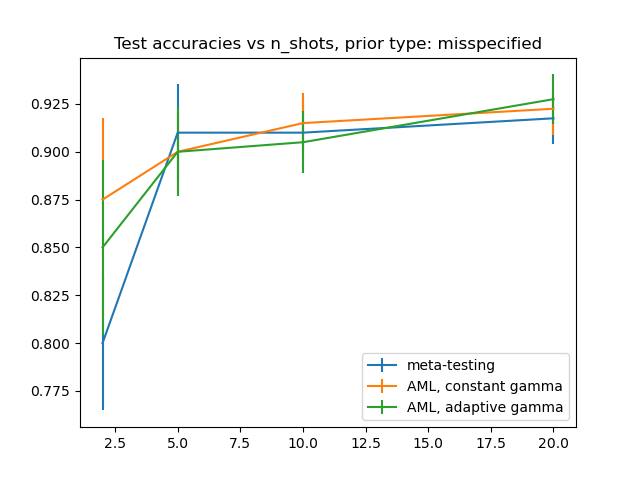
\includegraphics[width=\textwidth]{test_accuracies_model_misspecified}
		\caption{Test adaptation for a misspecified hyper-prior}	 	
	\end{subfigure}
	\hfill
	\caption{Average test accuracies for meta-adaptation with different values of $\gamma$. All runs assumed $\beta\rightarrow\infty$. Error bars represent standard errors from the average over 10 runs.}	 
	\label{fig:results-gamma}
\end{figure}

\begin{table}	
	
	\centering
	\begin{tabular}{lll}
		\toprule
		Method   & Hyper-prior  & Test accuracy   \\
		\midrule
		Meta-testing, 2-shot & correct   & $0.9\pm 0.037 $      \\
		Adapted meta-testing, 2-shot & correct   & $0.95\pm 0.039$      \\
		Adapted meta-testing with adaptive $\gamma$, 2-shot & correct   & $0.85\pm 0.042$      \\
		\midrule
		Meta-testing, 2-shot & misspecified   & $0.8\pm 0.035 $      \\
		Adapted meta-testing, 2-shot & misspecified   & $0.875\pm 0.043$      \\
		Adapted meta-testing with adaptive $\gamma$, 2-shot & misspecified   & $0.85\pm 0.046$    \\
		\midrule 
		
		Meta-testing, 5-shot & correct   & $0.92\pm 0.018 $      \\
		Adapted meta-testing, 5-shot & correct   & $0.93\pm 0.021$      \\
		Adapted meta-testing with adaptive $\gamma$, 5-shot & correct   & $0.96\pm 0.02$      \\
		\midrule
		Meta-testing, 5-shot & misspecified   & $0.91\pm 0.025 $      \\
		Adapted meta-testing, 5-shot & misspecified   & $0.9\pm 0.021$      \\
		Adapted meta-testing with adaptive $\gamma$, 5-shot & misspecified   & $0.9\pm 0.023$ \\   
		\midrule
		
		Meta-testing, 10-shot & correct   & $0.94\pm 0.012 $      \\
		Adapted meta-testing, 10-shot & correct   & $0.945\pm 0.011$      \\
		Adapted meta-testing with adaptive $\gamma$, 19-shot & correct   & $0.95\pm 0.01$      \\
		\midrule
		Meta-testing, 10-shot & misspecified   & $0.91\pm 0.016 $      \\
		Adapted meta-testing, 10-shot & misspecified   & $0.915\pm 0.016$      \\
		Adapted meta-testing with adaptive $\gamma$, 10-shot & misspecified   & $0.905\pm 0.01$    \\
		\midrule
		
		Meta-testing, 20-shot & correct   & $0.953\pm 0.012 $      \\
		Adapted meta-testing, 20-shot & correct   & $0.955\pm 0.012$      \\
		Adapted meta-testing with adaptive $\gamma$, 20-shot & correct   & $0.955\pm 0.011$      \\
		\midrule
		Meta-testing, 20-shot & misspecified   & $0.918\pm 0.013 $      \\
		Adapted meta-testing, 20-shot & misspecified   & $0.923\pm 0.014$      \\
		Adapted meta-testing with adaptive $\gamma$, 20-shot & misspecified   & $0.923\pm 0.013$    \\
		\midrule
		\bottomrule
	\end{tabular}
	\caption{Best test accuracies for the permuted-MNIST dataset with variable hyper-priors. All accuracies are averaged over 10 seeds and reported with standard error. Dashed line represents baseline meta-testing accuracy.}
	\label{table:gamma}
\end{table}

%TODO: explain findings

As we can see from Figure \ref{fig:results-gamma}, for the aligned hyper-prior, adaptive meta-learning offers some improvement over naive meta-testing. For the two-shot case adapting $\gamma$ did not improve results on average, and a deeper analysis showed that for several of the training seeds both the loss and gradients during meta-adaptation were large, thereby causing the loss estimation to be too noisy. 
For the misspecified hyper-prior, we see that choosing a constant value for $\gamma$ performed better in most settings. The misspecified hyper-prior caused the adaptive gamma to increase to rapidly, resulting in an ERM-like optimization process.

\section{Conclusions and future work}

% Something

\clearpage
\bibliographystyle{plainnat}
\bibliography{library}


\appendix
\section{Appendix}

\subsection{Hyper-parameters and implementation details} \label{append:hyper-params}
%TODO

\subsection{Basic properties of Gibbs posteriors} \label{append:gibbs-properties}

\begin{theorem} (\citet{Donsker1975} - variational formula)
	
	For any bounded function $f$:
	\begin{equation*} 
	\log \Expect{h\sim P}{e^{f(h)}}=\sup_{Q}\left[\Expect{h\sim Q}{e^{f(h)}}-D_{KL}(Q||P) \right ]
	\end{equation*}
	
	And the Gibbs posterior 
	$$Q(h)=\frac{P(h)e^{f(h)}}{\Expect{h\sim P}{e^{f(h)}}}$$ 
	Is the supremum with respect to $Q$.
\end{theorem}

\begin{proposition}
	The empirical Gibbs posterior 
	$$Q^\beta(h)=\frac{P(h)e^{-\beta \hat{\mathcal{L}}(h, S)}}{\Expect{h\sim P}{e^{-\beta \hat{\mathcal{L}}(h, S)}}}$$ 
	Is the minimizer of $$\min_{Q}\left[\hat{\mathcal{L}}(Q, S)+\frac{1}{\beta}D_{KL}(Q||P)\right ]$$
\end{proposition}

Additional useful properties:
\begin{enumerate}
	\item If $\beta=0$, we have $Q^\beta(h)=P(h)$
	\item If $\beta\rightarrow \infty$, then $Q$ is a delta function around the ERM solution $\min_h \hat{\mathcal{L}}(h,S)$
	\item $D_{KL}(Q^\beta||P)=-\beta\hat{\mathcal{L}}(Q^\beta, S)-\log\Expect{h\sim P}{e^{-\beta \hat{\mathcal{L}}(h, S)}}$
	\item $-\log\Expect{h\sim P}{e^{-\beta \hat{\mathcal{L}}(h, S)}}\leq \beta\hat{\mathcal{L}}(P,S)$ \footnote{Using Jensen's inequality}
	\item $Q^\beta$ is $DP(\frac{2\beta}{m})$ \citep{McSherry2007}
\end{enumerate}

\subsection{Useful log-moment bounds} \label{append:log-moment-stuff}
%TODO
\begin{theorem}
	If $l\in[a,b]$ is bounded and the prior $P$ is data-free, for any $\lambda\in \mathbb{R}$,
	$$\log \Expect{S\in \mathcal{D}, h\in P}{e^{\lambda(\hat{\mathcal{L}}(h,S)-\mathcal{L}(h,\mathcal{D}))}} \leq \frac{\lambda^2(b-a)^2}{8m}$$
\end{theorem}

\begin{theorem} \citep{Rivasplata2020}
	
	If $l\in[0,b]$ is bounded and the prior $P(h)\propto P_0(h)e^{-\beta\hat{\mathcal{L}}(h,S)}$ is an empirical Gibbs distribution, 
	$$\log \Expect{S\in \mathcal{D}, h\in P}{e^{\sqrt{m}(\hat{\mathcal{L}}(h,S)-\mathcal{L}(h,\mathcal{D}))}} \leq 2b^2(1+\frac{2\beta}{\sqrt{m}})+\log(1+e^{b^2/2})$$
\end{theorem}

\begin{theorem} \citep{Rivasplata2020, Dziugaite2018}
	
	If the prior P is $DP(\epsilon)$, and there exists some data-free prior $P^0$ such that with probability at least $1-\delta$,
	$$\Expect{h\sim Q_S}{f(S,h)} \leq D_{KL}(Q_S||P^0)+\log\frac{\zeta(m)}{\delta}$$
	then 
	$$\log \Expect{S\in \mathcal{D}, h\in P}{e^{f(S,h)}} \leq \log 2\zeta(m) + \frac{2\epsilon^2}{2}+\epsilon\sqrt{\frac{m}{2}\log(\frac{4}{\delta})}$$
	
	For $f=m\cdot kl(\hat{\mathcal{L}}(Q_S,S)||\mathcal{L}(Q_S,\mathcal{D}))$, the choice of $\zeta(m)=2\sqrt{m}$ is valid.
\end{theorem}

\begin{theorem} \citep{Rivasplata2020}
	
	For $w\in\mathbb{R}^d$ and prior $P(w)\propto e^{-\frac{\gamma\lambda}{2}||w||^2}$ where $\gamma>0$ and $\lambda>\max_i{\lambda_i-\hat{\lambda}_i}$ is the maximal difference between eigenvalues of the population covariance matrix and the sample covariance matrix,
	
	$$\log \Expect{S\in \mathcal{D}, w\in P}{e^{\gamma(\mathcal{L}(w,\mathcal{D})-\hat{\mathcal{L}}(w,S))}} = \gamma\max_w{\left [\mathcal{L}(w,\mathcal{D})-\hat{\mathcal{L}}(w,S)-(\lambda/2)||w||^2\right ]} + \frac{1}{2}\sum_{i=1}^{d}\log\left (\frac{\lambda}{\lambda+\hat{\lambda}_i-\lambda_i} \right ) $$
\end{theorem}

\begin{theorem} \citep{Rivasplata2020}
	
	If $l\in[0,\infty)$ is unbounded and the prior $P$ is data-free, for any $\lambda\in \mathbb{R}$,
	$$\log \Expect{S\in \mathcal{D}, h\in P}{e^{\lambda m(\hat{\mathcal{L}}(h,S)-\mathcal{L}(h,\mathcal{D}))}} \leq \frac{\lambda^2m}{2}\Expect{h\sim P}{l(h,Z)^2}$$
\end{theorem}

\subsection{Proof of the generic meta-adaptation bound} \label{append:proof-main-result}

We restate the result for stochastic kernels:

\begin{theorem} (PAC-Bayes for stochastic kernels - adapted from Theorem 2 in \citet{Rivasplata2020}) \label{thm:rivasplata-pb-appendix}
	Let $P\in \mathcal{K}(\mathcal{Z}^m, \mathcal{H})$ be a stochastic kernel, let $A: \mathcal{Z}^m\times \mathcal{H}\rightarrow \mathbb{R}^k$ be a measurable function for some positive integer $k$ and $F:\mathbb{R}^k\rightarrow \mathbb{R}$ be a convex function.
	Define $f\triangleq F\circ A$, and let 
	$$\xi(P_S, \mathcal{D}, f)=\int_{\mathcal{Z}^m}\int_{\mathcal{H}}e^{f(S, h)}P_S(dh)\mathcal{D}(dS)$$
	Such that $P_S$ is the distribution over $\mathcal{H}$ corresponding to the sampled $S$.
	
	Assuming $\xi(P_S, \mathcal{D}, f)$ is finite, for any $\delta \in (0,1)$, the following inequality holds uniformly for all posteriors $Q\in \mathcal{K}(\mathcal{Z}^m, \mathcal{H})$ with probability at least $1-\delta$ over the choice of $S\sim \mathcal{D}$:
	
	\begin{equation} \label{eq:ribasplata-pb-appendix}
	\Expect{h\sim Q_S}{f(S, h)} \leq D_{KL}(Q_S||P_S)+\log\left (\frac{\xi(P_S, \mathcal{D}, f)}{\delta}\right )
	\end{equation}
\end{theorem}

\begin{proposition}
	Let $\mathcal{Q}_{1:N}\in \mathcal{M}(\mathcal{M}(\mathcal{H}))$ be a meta-learned hyper-posterior (e.g. the result of meta-training on $\{S_1,...,S_N\}$), and let $\mathcal{D}_T\sim \tau$ be a \emph{given} test task. Let $Q: \mathcal{Z}^m\times\mathcal{M}(\mathcal{H})\rightarrow \mathcal{M}(\mathcal{H})$ be a given base learner. Let $l: \mathcal{H}\times \mathcal{Z}\rightarrow [0, 1]$ be a bounded loss function.
	For any $\delta_T \in (0,1)$, and for all $\lambda>0$, the following inequality holds uniformly for all hyper-posteriors $\mathcal{Q}\in \mathcal{M}(\mathcal{M}(\mathcal{H}))$ with probability at least $1-\delta_T$ over the draw of $S_T\sim \mathcal{D}_T$:
	
	\begin{align}
	\mathcal{L}(\mathcal{Q}, \mathcal{D}_T) \leq \hat{\mathcal{L}}(\mathcal{Q}, S_T) + \frac{1}{\lambda}D_{KL}(\mathcal{Q}||\mathcal{Q}_{1:N})
	+\frac{1}{\lambda}\log\frac{\tilde{\xi}(\lambda,\mathcal{Q}_{1:N},\mathcal{D}_T)}{\delta_T}
	\end{align}
	
	
	where 
	\begin{equation}\label{eq:tilde_xi}
	\tilde{\xi}(\lambda,\mathcal{Q}_{1:N},\mathcal{D}_T)\triangleq \Expect{S\sim \mathcal{D}_T, P\sim \mathcal{Q}_{1:N}, h\sim Q(P,S)}{e^{\lambda\left (\mathcal{L}(h, \mathcal{D}_T)-\hat{\mathcal{L}}(h, S)\right )}}
	\end{equation}
\end{proposition}

\begin{proof}
	First, we consider the setting of Theorem \ref{thm:rivasplata-pb-appendix} and extend it to meta-learning:
	
	We define a stochastic kernel for the 2-level hypothesis case as a pair $(\mathcal{P},P)\in \mathcal{K}(\mathcal{Z}^m, \mathcal{M}(\mathcal{H})\times \mathcal{H})$ such that for a given sample $S\in \mathcal{Z}^m$,  $(\mathcal{P},P')(S)$ is the distribution over $\mathcal{H}$ corresponding to sampling from the hyper-prior $P\sim \mathcal{P}(S)$ corresponding to $S$ and then sampling from $h\sim P'(S, P)$. For clarity, we denote these as distributions as $\mathcal{P}_S$ and $P'_{S,P}$
	
	Let $A: \mathcal{Z}^m\times \mathcal{H}\rightarrow \mathbb{R}^k$ be a measurable function for some positive integer $k$ and $F:\mathbb{R}^k\rightarrow \mathbb{R}$ be a convex function.
	Define $f\triangleq F\circ A$, and let 
	$$\xi((\mathcal{P}_S,P'_S), \mathcal{D}, f)=\int_{\mathcal{Z}^m}\int_{\mathcal{M}(\mathcal{H})\times\mathcal{H}}e^{f(S, h)}\mathcal{P}_S\times P'_{S,P}(dP,dh)\mathcal{D}(dS)$$
	\RM{Shouldn't there be $3$ integrals rather than $2$? The notation $P_S(P)(dh)$ is somewhat cumbersome.} \LF{Is this new version clearer?}
	
	Using Equation \ref{eq:ribasplata-pb-appendix} with $f(S,(P,h))=\lambda(\mathcal{L}(h,\mathcal{D})-\hat{\mathcal{L}}(h,S))$, a 2-level posterior $(\mathcal{Q}_S, Q_S)$ and a 2-level prior $(\mathcal{Q}_{1:N}, Q_S)$,
	we have that for any $\delta_T \in (0,1)$, the following inequality holds uniformly for all posteriors $Q\in \mathcal{K}(\mathcal{Z}^m, \mathcal{H})$ with probability at least $1-\delta_T$ over the choice of $S_T\sim \mathcal{D}_T$:
	
	\begin{equation} \label{eq:appendix-proof-eq}
	\begin{split}
	\Expect{h\sim (\mathcal{Q}_{S_T}, Q_{S_T})}{\lambda(\mathcal{L}(h,\mathcal{D}_T)-\hat{\mathcal{L}}(h,S_T))} &\leq D_{KL}((\mathcal{Q}_{S_T}, Q_{S_T})||(\mathcal{Q}_{1:N}, Q_{S_T}))\\
	&+\log\left (\frac{\xi\left ((\mathcal{Q}_{1:N}, Q_S), \mathcal{D}_T, \lambda(\mathcal{L}(h,\mathcal{D})-\hat{\mathcal{L}}(h,S))\right )}{\delta_T}\right )
	\end{split}
	\end{equation}
	
	It is important to note that the only assumption we make here is that the hyper-prior $\mathcal{Q}_{1:N}$ is data-free with respect to the new data $S_T\sim \mathcal{D}_T$. Since we consider meta-learned distributions over priors, this is a reasonable assumption, as it is satisfied if we have not seen $S_T$ during meta-training.
	
	First, let us make sure that the moment terms are equivalent. We note here that since the hyper-prior does not depend on $S_T$, the expectation can be easily decomposed as follows:
	
	\begin{align*}
	\begin{split}
		\xi\left ((\mathcal{Q}_{1:N}, Q_S), \mathcal{D}_T, \lambda(\mathcal{L}(h,\mathcal{D})-\hat{\mathcal{L}}(h,S))\right )
		&=\int_{\mathcal{Z}^m}\int_{\mathcal{H}}e^{\lambda\left (\mathcal{L}(h, \mathcal{D}_T)-\hat{\mathcal{L}}(h, S)\right )}\mathcal{Q}_{1:N}(dP)Q(P,S)(dh)\mathcal{D}_T(dS)\\
		&=\Expect{S\sim \mathcal{D}_T, P\sim \mathcal{Q}_{1:N}, h\sim Q(P,S)}{e^{\lambda\left (\mathcal{L}(h, \mathcal{D}_T)-\hat{\mathcal{L}}(h, S)\right )}}\\
		&\triangleq \tilde{\xi}(\lambda,\mathcal{Q}_{1:N},\mathcal{D}_T)
	\end{split}
	\end{align*}
	
	Substituting this in Equation \ref{eq:appendix-proof-eq} and moving terms, we get (with probability at least $1-\delta_T$ over the draw of $S_T\sim \mathcal{D}_T$):
	
	\begin{equation} 
	\begin{split}
	\Expect{h\sim (\mathcal{Q}_{S_T}, Q_{S_T})}{\mathcal{L}(h,\mathcal{D}_T)} &\leq \Expect{h\sim (\mathcal{Q}_{S_T}, Q_{S_T})}{\hat{\mathcal{L}}(h,S_T)} +\frac{1}{\lambda} D_{KL}((\mathcal{Q}_{S_T}, Q_{S_T})||(\mathcal{Q}_{1:N}, Q_{S_T}))\\
	&+\frac{1}{\lambda}\log\left (\frac{\tilde{\xi}(\lambda,\mathcal{Q}_{1:N},\mathcal{D}_T)}{\delta_T}\right )
	\end{split}
	\end{equation}
	
	By definition, this is equivalent to writing:
	
	\begin{equation} \label{eq:appendix-proof-eq-2}
	\mathcal{L}(\mathcal{Q}_{S_T},\mathcal{D}_T) \leq \hat{\mathcal{L}}(\mathcal{Q}_{S_T},S_T) +\frac{1}{\lambda} D_{KL}((\mathcal{Q}_{S_T}, Q_{S_T})||(\mathcal{Q}_{1:N}, Q_{S_T}))+\frac{1}{\lambda}\log\left (\frac{\tilde{\xi}(\lambda,\mathcal{Q}_{1:N},\mathcal{D}_T)}{\delta_T}\right )
	\end{equation}
	
	For the KL-divergence expression, we apply a standard KL decomposition:
	
	\begin{align*}
	\begin{split}
	D_{KL}((\mathcal{Q}_{S_T}, Q_{S_T})||(\mathcal{Q}_{1:N}, Q_{S_T}))&=\Expect{(P,h)\sim (\mathcal{Q}_{S_T},Q_{S_T})}{\log\frac{\mathcal{Q}_{S_T}(P)Q(P, S_T)(h)}{\mathcal{Q}_{1:N}(P)Q(P, S_T)(h)}}\\
	&=\mathbb{E}_{P\sim \mathcal{Q}_{S_T}}\Expect{h\sim Q(P,S_T)}{\log\frac{\mathcal{Q}_{S_T}(P)Q(P, S_T)(h)}{\mathcal{Q}_{1:N}(P)Q(P, S_T)(h)}}\\
	&=\Expect{P\sim \mathcal{Q}_{S_T}}{\log\frac{\mathcal{Q}_{S_T}(P)}{\mathcal{Q}_{1:N}(P)}}+\mathbb{E}_{P\sim \mathcal{Q}_{S_T}}\Expect{h\sim Q(P,S_T)}{\log\frac{Q(P, S_T)(h)}{Q(P, S_T)(h)}}\\
	&=\Expect{P\sim \mathcal{Q}_{S_T}}{\log\frac{\mathcal{Q}_{S_T}(P)}{\mathcal{Q}_{1:N}(P)}}\\
	&=D_{KL}(\mathcal{Q}_{S_T}||\mathcal{Q}_{1:N})
	\end{split}
	\end{align*}
	
	Finally, combining this result with Equation \ref{eq:appendix-proof-eq-2} gives us the final inequality:
	
	For any $\delta_T \in (0,1)$, the following holds uniformly for all hyper-posteriors $\mathcal{Q}_{S_T}\in \mathcal{M}(\mathcal{M}(\mathcal{H}))$ with probability at least $1-\delta_T$ over the draw of $S_T\sim \mathcal{D}_T$:
	
	\begin{align*}
	\mathcal{L}(\mathcal{Q}_{S_T}, \mathcal{D}_T)) \leq \hat{\mathcal{L}}(\mathcal{Q}_{S_T}, S_T) + \frac{1}{\lambda}D_{KL}(\mathcal{Q}_{S_T}||\mathcal{Q}_{1:N})
	+\frac{1}{\lambda}\log\frac{\tilde{\xi}(\lambda,\mathcal{Q}_{1:N},\mathcal{D}_T)}{\delta_T}
	\end{align*}
	\end{proof}

\subsection{Optimal hyper-parameters for Gibbs meta-adaptation} \label{append:optimiziation}

\subsubsection{Optimizing $\gamma$}

Deriving Equation \ref{eq:pb-adapt-multi} by $\gamma$ gets us:

\begin{equation} \label{eq:gamma-deriv}
(1-\frac{\gamma}{\lambda})\frac{d}{d\gamma}\hat{\mathcal{L}}_{aml} -\frac{1}{\lambda}\hat{\mathcal{L}}_{aml} +\frac{1}{\lambda}\hat{\mathcal{L}}_{ml} =0
\end{equation}

We must calculate the derivative of the expected loss (we mark $Q\triangleq Q(P,S_T)$ for brevity): 

$$\frac{d}{d\gamma}\hat{\mathcal{L}}_{aml}=\int \frac{d}{d\gamma}\mathcal{Q}_{1:N,T}(P)\hat{\mathcal{L}}(Q, S_T)dP=\int \mathcal{Q}_{1:N}(P)\hat{\mathcal{L}}(Q, S_T)\frac{d}{d\gamma}
\frac{e^{-\gamma\hat{\mathcal{L}}(Q,S_T)}}{\Expect{P\sim \mathcal{Q}_{1:N}}{e^{-\gamma\hat{\mathcal{L}}(Q,S_T)}}}dP$$

$$=\int \mathcal{Q}_{1:N}(P)\hat{\mathcal{L}}(Q, S_T)\frac{-\hat{\mathcal{L}}(Q,S_T)e^{-\gamma\hat{\mathcal{L}}(Q,S_T)}\Expect{P\sim \mathcal{Q}_{1:N}}{e^{-\gamma\hat{\mathcal{L}}(Q,S_T)}}
	-e^{-\gamma\hat{\mathcal{L}}(Q,S_T)}\Expect{P\sim \mathcal{Q}_{1:N}}{-\hat{\mathcal{L}}(Q,S_T)e^{-\gamma\hat{\mathcal{L}}(Q,S_T)} }}{\Expect{P\sim \mathcal{Q}_{1:N}}{e^{-\gamma\hat{\mathcal{L}}(Q,S_T)}}^2}dP$$


$$=\int \mathcal{Q}_{1:N,T}(P)\hat{\mathcal{L}}(Q, S_T)\left (-\hat{\mathcal{L}}(Q,S_T)-
\frac{\Expect{P\sim \mathcal{Q}_{1:N}}{-\hat{\mathcal{L}}(Q,S_T)e^{-\gamma\hat{\mathcal{L}}(Q,S_T)} }}{\Expect{P\sim \mathcal{Q}_{1:N}}{e^{-\gamma\hat{\mathcal{L}}(Q,S_T)}}}\right)dP$$

To conclude our calculation of the derivative, we get:

$$\frac{d}{d\gamma}\hat{\mathcal{L}}_{aml}=-\Expect{P\sim \mathcal{Q}_{1:N,T}}{\hat{\mathcal{L}}(Q,S_T)^2}-\frac{\Expect{P\sim \mathcal{Q}_{1:N}}{-\hat{\mathcal{L}}(Q,S_T)e^{-\gamma\hat{\mathcal{L}}(Q,S_T)} }}{\Expect{P\sim \mathcal{Q}_{1:N}}{e^{-\gamma\hat{\mathcal{L}}(Q,S_T)}} }\hat{\mathcal{L}}_{aml} $$

Marking $R(\gamma)=\frac{\Expect{P\sim \mathcal{Q}_{1:N}}{\hat{\mathcal{L}}(Q,S_T)e^{-\gamma\hat{\mathcal{L}}(Q,S_T)} }}{\Expect{P\sim \mathcal{Q}_{1:N}}{e^{-\gamma\hat{\mathcal{L}}(Q,S_T)}} }$ for convenience, we use Equation \ref{eq:gamma-deriv} and replace the derivatives with this expression to find the optimal value of $\gamma$: 

\begin{align*} 
\begin{split}
&(\lambda-\gamma)\left (-\Expect{P\sim \mathcal{Q}_{1:N,T}}{\hat{\mathcal{L}}(Q,S_T)^2}+R(\gamma)\hat{\mathcal{L}}_{aml}\right )\\& - \hat{\mathcal{L}}_{aml}+\hat{\mathcal{L}}_{ml} = 0
\end{split}
\end{align*}

\begin{align*} 
\begin{split}
-(\lambda-\gamma) = \frac{\hat{\mathcal{L}}_{aml}-\hat{\mathcal{L}}_{ml}}{\Expect{P\sim \mathcal{Q}_{1:N,T}}{\hat{\mathcal{L}}(Q,S_T)^2}-R(\gamma)\hat{\mathcal{L}}_{aml}}
\end{split}
\end{align*}

\begin{align} \label{eq:meta-pb-gamma}
\begin{split}
\gamma = \lambda+\frac{\hat{\mathcal{L}}_{aml}-\hat{\mathcal{L}}_{ml}}{\Expect{P\sim \mathcal{Q}_{1:N,T}}{\hat{\mathcal{L}}(Q,S_T)^2}-R(\gamma)\hat{\mathcal{L}}_{aml}}
\end{split}\hfill
\end{align}

\subsubsection{Optimizing $\lambda$}

Deriving Equation \ref{eq:pb-adapt-multi} by $\lambda$ gets us:

$$\frac{\gamma}{\lambda^2} \hat{\mathcal{L}}_{aml}-\frac{\gamma}{\lambda^2}\hat{\mathcal{L}}_{ml}-\frac{1}{\lambda^2}\log\frac{\xi(\mathcal{Q}_{1:N}\lambda)}{\delta_T}+\frac{1}{\lambda}\frac{d}{d\lambda}\log\xi(\mathcal{Q}_{1:N},\lambda)=0$$

Multiplying by $\lambda^2$ gives:

$$\gamma \hat{\mathcal{L}}_{aml}-\gamma\hat{\mathcal{L}}_{ml}-\log\frac{\xi(\mathcal{Q}_{1:N}\lambda)}{\delta_T}+\lambda\frac{d}{d\lambda}\log\xi(\mathcal{Q}_{1:N},\lambda)=0$$

Since 
$$\frac{d}{d\lambda}\log\xi(\mathcal{Q}_{1:N},\lambda)=\frac{\Expect{P\sim \mathcal{Q}_{1:N},S\sim D,h\sim Q(P,S_T)}{(\mathbb{E}_S\hat{L}(h, S)-\hat{L}(h, S))e^{\lambda(\mathbb{E}_S\hat{L}(h, S)-\hat{L}(h, S))} }}{\Expect{P\sim \mathcal{Q}_{1:N},S\sim D,h\sim Q(P,S_T)}{e^{\lambda(E_S\hat{L}(h, S)-\hat{L}(h, S)} }}\triangleq R_\xi(\lambda)$$

We can write the above equation as:

$$\gamma(\hat{\mathcal{L}}_{aml}-\hat{\mathcal{L}}_{ml})-\log\frac{\xi(\mathcal{Q}_{1:N},\lambda)}{\delta_T}=-\lambda R_\xi(\lambda)$$

meaning,

\begin{align} \label{eq:meta-pb-lambda}
\begin{split}
\lambda = \frac{\gamma(\hat{\mathcal{L}}_{ml}-\hat{\mathcal{L}}_{aml})+\log\frac{\xi(\mathcal{Q}_{1:N},\lambda)}{\delta_T}}{R_\xi(\lambda)}
\end{split}
\end{align}

The first term of the numerator serve encourages a lower value for $\lambda$ if there is a positive prediction gain from meta-adaptation $\hat{\mathcal{L}}_{aml}<\hat{\mathcal{L}}_{ml}$. This is not immediately intuitive as we would expect that a low empirical loss would encourage more distance from the hyper-prior and therefore higher $\lambda$. The moment term $\xi(\mathcal{Q}_{1:N}, \lambda)$ increases with $\lambda$, so choosing a very large value for it may cause the moment to diverge and therefore violate the base conditions for the data-dependent (Theorem \ref{thm:rivasplata-pb}). 

%\subsection{Optimizing $\beta$}
%
%Finally, while $\beta$ does not appear explicitly in Equation \ref{eq:pb-adapt-multi}, it is still possible to derive by it as it appears in our losses:
%
%$$(1-\frac{\gamma}{\lambda})\frac{d}{d\beta}\hat{\mathcal{L}}_{aml}+\frac{\gamma}{\lambda}\frac{d}{d\beta}\hat{\mathcal{L}}_{ml}+
%\frac{1}{\lambda}\frac{d}{d\beta}ln\xi(\mathcal{Q}_{1:N},\lambda)=0$$
%
%As we can see, this equation has no explicit dependence on $\beta$, and so extracting a meaningful implicit equation for $\beta$ that is not strongly linked to the base learner $Q$ is impossible.

\subsection{Hyper-priors with Gibbs base learners are differentially-private} \label{append:proof-dp}

\begin{proposition} \label{thm:pair-is-dp-appendix}
	Let $\mathcal{P}\in \mathcal{M}(\mathcal{M}(\mathcal{H}))$ be a hyper-prior.
	Let $l:\mathcal{H}\times \mathcal{Z}\rightarrow [0,1]$ be a bounded loss function.
	
	If the base learner $Q\in \mathcal{M}(\mathcal{H})$ is the Gibbs posterior $Q(P, S)(h)\propto P(h)e^{-\beta\hat{\mathcal{L}}(h, S)}$, 
	then the pair hypothesis $(\mathcal{P}, Q)$ satisfies $DP\left (\frac{2\beta}{m}\right )$.
\end{proposition}

\begin{proof}
	From Theorem 6 in \citet{McSherry2007}, the Gibbs posterior $Q(P, S)(h)$ satisfies $DP\left (2\beta\Delta L\right )$, where $\Delta L$ is the the largest possible difference  $sup_{h\in\mathcal{H}}\hat{\mathcal{L}}(h,S)-\hat{\mathcal{L}}(h,S')$ for $S,S'$ that differ by one example. Since the loss is bounded in $[0,1]$ and $S,S'$ are of size $m$, we have $\Delta L\leq \frac{1}{m}$, and so the base learner $Q(P, S)(h)$ satisfies $DP\left (\frac{2\beta}{m}\right )$.
	
	
	It remains to prove that for all $(A_1,A_2)\in (\mathcal{M}(\mathcal{M}(\mathcal{H})), \mathcal{M}(\mathcal{H}))$, 
	$$ \frac{\mathcal{P}(S, A_1)Q(S,A_2)}{\mathcal{P}(S', A_1)Q(S',A_2)}\leq e^{\frac{2\beta}{m}}$$
	
	From the DP property, 
	
	$$ \frac{\mathcal{P}(S, A_1)Q(S,A_2)}{\mathcal{P}(S', A_1)Q(S',A_2)}\leq \frac{\mathcal{P}(S, A_1)}{\mathcal{P}(S', A_1)}e^{\frac{2\beta}{m}}$$
	
	Since $\mathcal{P}$ is a hyper-prior, we assume it is data-free with respect to $S$, and so 
	$$\mathcal{P}(S, A_1)=\mathcal{P}(S', A_1)=\mathcal{P}(A_1)$$
	
\end{proof}


\end{document}